\part{Praktischer Teil}
%Nachdem im theoretischen Teil die Grundlagen probabilistischer Vorhersagen, Ensemblevorhersagen sowie geeignete Evaluationsmethoden vorgestellt wurden, erfolgt nun die A-Anwendung auf Temperaturvorhersagen. Zunächst wird die Datengrundlage genauer erläutert.


\chapter{Numerische Wettervorhersagemodelle} \label{chap:nwp}
In diesem Teil werden die im theoretischen Teil vorgestellten Methoden zur Evaluation probabilistischer Vorhersagen auf das Beispiel probabilistischer Temperaturvorhersagen angewendet. Dazu wird zunächst in diesem Kapitel erläutert, nach welchem Prinzip Wettervorhersagen erstellt werden, wie daraus die Grundlagen für probabilistische Temperaturvorhersagen entstehen können sowie welche Art der Verifikationsdaten sich eignen.

\section{Grundlagen}
Numerische Wettervorhersagemodelle modellieren deterministisch auf Basis einer Vielzahl an Differentialgleichungen den zukünftigen Zustand der Atmosphäre und der Erdoberfläche \parencite{dwd_numerische_vorhersagemodelle}. Dabei werden wichtige atmosphärische Variablen wie Luftbewegung, Luftdruck, einfallende Sonnenstrahlung, Wasserverdunstung, Wolkenbildung, Erwärmung der Erdoberfläche sowie Temperaturausgleich berücksichtigt. Diese Prozesse stehen in engem Zusammenhang miteinander und können auf Basis physikalischer und chemischer Gesetzmäßigkeiten mathematisch formuliert werden.

Das Lösen dieser komplexen Modellierungsgleichungen geschieht am Computer unter hohem Rechenaufwand mit numerischen Verfahren \parencite{DWD_wie_entsteht}. Dazu wird der modellierte Bereich mit einem horizontalen Gitter mit mehreren Vertikalen Schichten diskretisiert. Die Berechnung erfolgt entweder an den Gitterpunkten oder für die einzelnen Gitterzellen. Die in den Gitterzellen vorhergesagten Größen können dann als Mittelwert der horizontalen Fläche der Zelle zur jeweiligen vertikalen Schicht interpretiert werden \parencite{reinert2025icon_dwd}.


\section{Global- und Lokalmodelle}
Die Genauigkeit eines Modells hängt unter anderem von dessen horizontaler Auflösung ab. Eine hohe Auflösung ermöglicht eine feinere Abbildung der Entwicklung der Atmosphäre. Dadurch können Modellvorhersagen präziser und räumlich spezifischer werden \parencite{DWD_wie_entsteht}. 

Jedoch führt eine höhere Auflösung dazu, dass das Modell mehr Punkte berechnen muss \parencite{DWD_wie_entsteht}. Diesen Tradeoff zwischen Vorhersagegenauigkeit und Rechenaufwand gilt es zu berücksichtigen. Jedoch unterscheiden sich Modelle  nicht nur in ihrer Auflösung, sondern auch in der Größe des Gebietes, das sie abdecken. Aquivalent zur Auflösung gilt: Je größer das Modellgebiet, desto höher der Rechenaufwand.

Will man beispielsweise das Wetter für einen Zeitraum von mehreren Tagen in Meck\-lenburg-Vor\-pommern vorhersagen, reicht ein Modell, das ausschließlich das Bundesland abbildet, nicht aus. Es benötigt auch Informationen aus Bereichen außerhalb des Modellgebiets. Es könnte sich etwa von Weitem ein Tiefdruckgebiet nähern, dessen Einfluss berücksichtigt werden muss, damit die Vorhersage realistisch bleibt.

Das bedeutet, dass für längere Vorhersagezeiträume größere räumliche Bereiche beachtet werden müssen. Gleichzeitig benötigen ortsspezifische Vorhersagen ein sehr fein aufgelöstes Gitter. Um die Rechenanforderungen dennoch im Rahmen zu halten, werden daher Global- und Lokalmodelle kombiniert genutzt \parencite{DWD_wie_entsteht}. Ein Globalmodell modelliert den Zustand der Atmosphäre der gesamten Erde auf einem gröberem Gitter und informiert ein höher aufgelöstes Lokalmodell mit Randbedingungen \parencite{reinert2025icon_dwd}. So hat das Lokalmodell Zugriff auf Veränderungen außerhalb seines Modellbereichs und liefert trotzdem hoch aufgelöste Vorhersagen. 
% Konvektion, konvektiven Skala, Parametrisierung

\section{Ensemble Vorhersagen}
Mathematisch kann man die numerische Wettervorhersage als Anfangswertproblem auffassen. Entsprechend ist ein entscheidender erster Schritt in der Vorhersage der Atmosphäre, ihre Zustände bei Vorhersagebeginn zu erfassen. Das Bereitstellen dieser Anfangswerte ist die Aufgabe der Meteorologischen Datenassimilation \parencite{wergen2002datenassimilation}. Dafür werden eine Vielzahl an Beobachtungsdaten verwendet. Diese kommen beispielsweise von Flugzeugen, Bojen, Satelliten, Wetterstationen und Radiosonden. Solche Daten reichen jedoch alleine nicht aus, um die Anfangszustände zu bestimmen. Auch vorherige Daten sowie die Vorhersagen des Modells selbst, werden bei der Bestimmung berücksichtigt. 

Die Datenassimilation ist jedoch mit Unsicherheiten verbunden \parencite{wergen2002datenassimilation}. Das liegt unter anderem daran, dass sowohl die Beobachtungen als auch die Modellvorhersagen fehlerbehaftet sind und die verfügbaren Beobachtungen räumlich und zeitlich lückenhaft vorliegen. Die Atmosphäre ist außerdem ein chaotisches System; schon minimale Ungenauigkeiten in den Anfangsbedingungen können über die Zeit zu sehr verschiedenen Ergebnissen führen \parencite{dwd_ensemble_vorhersage}. So können zwei Modelldurchläufe mit leicht unterschiedlichen Anfangswerten völlig verschiedene, aber dennoch plausible, Wetterszenarien produzieren. Um solche Unsicherheiten abzubilden, werden Ensemblevorhersagen genutzt \parencite{dwd_ensemble_vorhersage}. Dabei simuliert ein Modell die Atmosphäre auf der Grundlage von verschiedenen realistischen Anfangswerten oder leicht veränderten Modellparametern \footnote{Genaugenommen ist das die Funktionsweise eines single-model Ensemble. Es gibt auch multi-model Ensemble. Bei ihnen bilden verschiedene Modelle die Ensemblemitglieder,}. Dadurch erhält man eine Reihe plausibler Vorhersagen, die Ensemblemitglieder.

Aus den Ensemblemitglieder lassen sich probabilistische Vorhersagen ableiten. Dazu können wir unter anderem statistische Postprocessing Methoden verwenden (siehe Abschnitt \ref{sec:postproc}).

\section{Verifikationsdaten für Modellvorhersagen}
Zur Evaluation von Vorhersagen und zum Training von Postprocessing Verfahren benötigen wir Daten, die die tatsächlichen Wetterbedingungen möglichst gut abbilden, um Vorhersagen zuverlässig bewerten bzw. erstellen zu können. Für die Auswahl solcher Verifikations- bzw. Trainingsdaten  gibt es grundsätzlich mehrere Möglichkeiten.  

Der klassische Ansatz ist, Beobachtungen an Wetterstationen zu verwenden \parencite{gneiting2014calibration,feldmannGridStationBasedPostprocessing2019}. Dazu werden die Ausgaben von numerischen Wettervorhersagemodellen mittels Interpolation auf die jeweiligen punktuellen Stationsstandorte übertragen und anschließend evaluiert. Das Ziel ist also, Vorhersagen für genau die meteorologischen Größen zu verbessern bzw. zu bewerten, die wir direkt beobachten.

Eine alternative Möglichkeit besteht in der Nutzung von Reanalysedaten \parencite{gneiting2014calibration,feldmannGridStationBasedPostprocessing2019}. Dabei werden retrospektiv Wettermodelle unter Einbezug bekannter Atmosphärenparametern erneut gerechnet. Der Vorteil dieses Ansatzes liegt darin, dass das räumliche und zeitliche Gitter den Modellgitterdaten entspricht und somit jede Zelle ohne Interpolation direkt bewertet werden kann. Ein Nachteil ist jedoch, dass nicht für jedes Wettermodell passende Reanalysedatensätze verfügbar sind.

In der vorliegenden Arbeit verwenden wir einen dritten Ansatz, der eine Mischung aus den vorherigen Ansätze darstellt. Anstelle von Reanalysen verwenden wir einen beobachtungsbasierten Referenzgitterdatensatz. Hierbei wird ein Gitter durch statistische Interpolationsverfahren aus unterschiedlichen Beobachtungsquellen erzeugt. Die Schwierigkeit besteht darin, dass sich Vorhersagemodell und Referenzdatensatz in Projektion und Gitterstruktur unterscheiden können. Daher ist, analog zum Vorgehen bei Stationsdaten, eine geeignete Interpolation bzw. ein Regridding erforderlich, um die Daten auf ein gemeinsames räumliches Raster zu überführen.

Der entscheidende Vorteil gegenüber Reanalysen ist die Verfügbarkeit, gegenüber Stationsbeobachtungen das Gitterformat. Ein wesentlicher Nachteil dieses Ansatzes ist, dass der Referenzdatensatz selbst systematische Fehler enthalten kann, da er auf interpolierten und teilweise modellbasierten Informationen beruht. 
\newpage


\chapter{Datengrundlage} \label{chap:data}
In diesem Kapitel stellen wir die Datengrundlage für den praktischen Teil der Arbeit vor. Als zu prognostizierenden Wetterparameter betrachten wir die 2-m-Temperatur. Sie beschreibt Lufttemperatur in 2 Metern Höhe über dem Boden \parencite{dwd_2m_temperatur}.

Für eine Vorhersagevaluation sind dabei zwei DWD-Datensätze entscheidend: Die Modellvorhersagen eines Ensemblemodells, auf dessen Grundlagen wir die probabilistischen Vorhersagen erstellen und der Verifikationsdatensatz mit dem wir diese Vorhersagen überprüfen. Diese stellen wir in den Abschnitten \ref{sec:icon} und \ref{sec:host} vor. Anschließend zeigen wir in den Abschnitten \ref{sec:proj} bis \ref{sec:indx}, wie wir aus diesen Datensätzen die für die vorliegende Arbeit verwendeten Ausschnitt aus diesen Daten ableiten. Dabei beschreiben und begründen wir die getroffene Auswahl und führen eine einheitliche Notation der Daten ein. Abschließend beschreiben wir den in der vorliegenden Arbeit verwendeten Ausschnitt aus diesen Daten in Abschnitt \ref{sec:desc} zusammen.

\section{Modelldaten: ICON-D2-EPS} \label{sec:icon}
Das ICON-D2-EPS ist ein numerisches Wettervorhersagemodell des Deutschen Wetterdienstes (DWD) mit 20 Ensemblemitgliedern \parencite{reinert2025icon_dwd}. Es handelt es sich um ein Lokalmodell des Globalmodells ICON-EPS für den Raum Deutschland, Schweiz, Österreich und Teile der anderen anliegenden Länder. Das modellierte Gebiet ist auf einem R19B07 Dreiecksgitter aus 542040 Gitterpunkten pro Schicht abgebildet mit mittlerer horizontalen Auflösung von 2,1 $\mathrm{km}^2$ pro Dreieck \parencite{reinert2025icon_dwd}. Beginnend bei 00:00 UTC wird alle drei Stunden eine neue stündliche 0- bis 48-Stunden-Vorhersage gerechnet. Abbildung \ref{fig:icon} zeigt die Vorhersage eines Ensemblemitglieds für einen Zeitpunkt.

Die ICON-D2-EPS Modellvorhersagedaten wurden über das Pamore (PArallel MOdel data REtrieve from Oracle databases) Webinterface abgerufen. Es ist ein Webinterface des DWD zur Entarchivierung und Bereitstellung historischer Daten numerischer Wettervorhersagemodelle für Forschung und öffentliche Einrichtungen \parencite{TUTORIALICON2025,dwd_pamore}. Für die Nutzung ist ein Benutzeraccount erforderlich, welcher über die Universität Greifswald gestellt wurde. Nach Anmeldung über \url{https://webservice.dwd.de/cgi-bin/spp1167/webservice.cgi} können Datenbankabfragen entweder direkt über ein Textfeld eingegeben oder über ein webbasiertes Formular schrittweise erstellt werden. Nach dem Absenden der Abfrage werden die angeforderten Modelldaten extrahiert und auf einem FTP-Server des DWD zum Download bereitgestellt.
Beispielsweise liefert die Abfrage
\begin{lstlisting}
pamore -G -F -d 2025112500 -hstart 0 -hstop 48 -hinc 1 -tflag best -ee T_2M%HG -epsmember 1-20 -ires r19b07 -model ilam+eps
\end{lstlisting}
für den Vorhersagedurchlauf des ICON-D2-EPS vom 25.10.2025 00:00 UTC, für alle 20 Ensemblemitglieder und Vorhersagehorizonte $0\text{-}48\h$ die  2-m-Temperatur Vorhersage. Jede Kombination aus Ensemblemitglied und Zeitschritt ergibt eine Datei. Dadurch ergeben sich für dieses Beispiel $20 \times 49 = 980$ Dateien. Diese sind im GRIB2-Format abrufbar, einem von der Weltorganisation für Meteorologie (WMO) standardisierten Format zur Übertragung meteorologischer Gitterdaten \parencite{DWD_GRIB2}. 

Die GRIB2-Dateien beinhalten lediglich die Vorhersagedaten. Um die Beschreibung des ICON-Modellgitters zu erhalten, benötigen wir eine separate NetCDF Datei, die diese Information enthält und so die räumliche Zuordnung der Datenpunkte ermöglicht.
Diese ist über den Open-Data Server des DWD über 
\begin{quote}
    \url{https://opendata.dwd.de/weather/lib/cdo/}
\end{quote}
abrufbar. Generell stellt der DWD über seinen Open-Data-Server eine Vielzahl weiterer Wetter- und Klimainformationen bereit. Auch ICON-Modellvorhersagen sind prinzipiell über den Server verfügbar, allerdings werden die Daten eines Tages durch nachfolgende Aktualisierungen überschrieben, sodass sie nur temporär abrufbar sind.

\begin{figure}[h!]
\centering
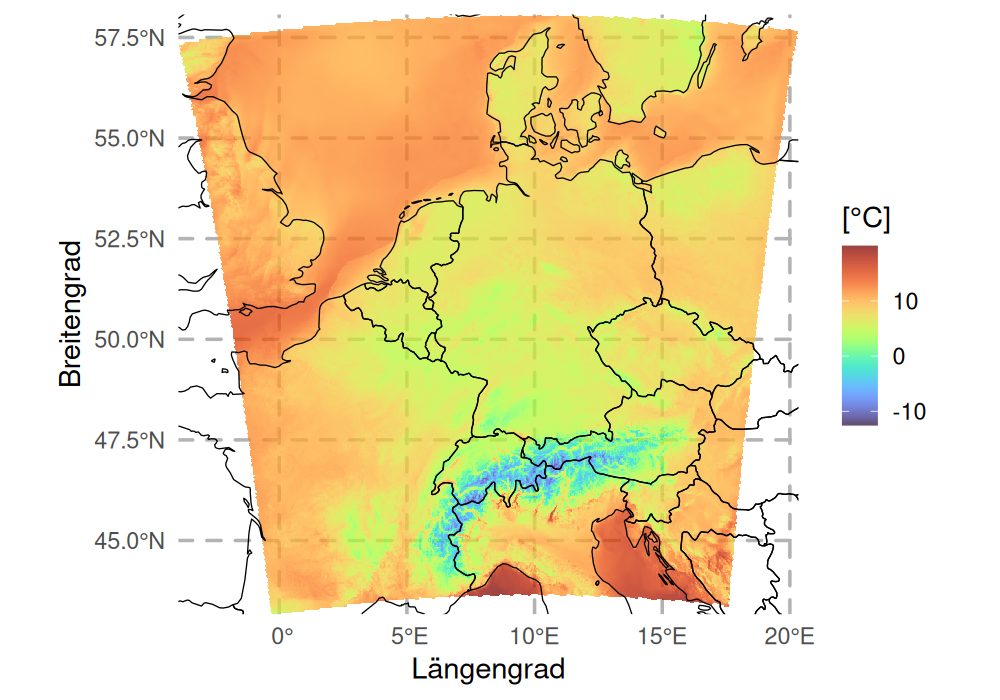
\includegraphics[width=0.8\linewidth]{figs/icon_region_Rplot.png}
\caption{Modellgebiet ICON-D2-EPS auf einem regulären Lat/Lon-Gitter dargestellt. Abgebildet ist die 0h (instant) 2-m-Temperatur Vorhersage des 1. Ensemblemitglieds vom 3.11.2025 06:00 UTC.}
\label{fig:icon}
\end{figure}

\section{Verifikationsdaten: HOSTRADA} \label{sec:host}
HOSTRADA ist ein Akronym für hochaufgelösten stündlichen Rasterdatensatz \parencite{krahenmann_high-resolution_2018,dwd_hostrada_beschreibung}. Es handelt sich um einen Referenzdatensatz für Deutschland des DWD, der seit 1995 stündlich meteorologische Parameter in der Lambert-Conformal-Conic-Projektion (LCC, EPSG:3034) mit einer horizontalen Auflösung von $1\times1\ \mathrm{km^2}$ bereitstellt. Die Daten ergeben sich aus der Interpolation von Stationsdaten unter Einbezug von Satelliten- und Modelldaten. $720 \times 938 = 333404$ Gitterpunkte sind mit Werten belegt. Das Modellgebiet ist in Abbildung \ref{fig:hostrada} dargestellt.

Die HOSTRADA 2-m-Temperaturdaten stammen genau wie die ICON-\-Modell\-gitter\-be\-schreibung aus dem Open-Data-Angebot des Deutschen Wetterdienstes und sind über
\begin{quote}
    \url{https://opendata.dwd.de/climate_environment/CDC/grids_germany/hourly/hostrada/air_temperature_mean/}
\end{quote}
abrufbar. Eine Datei umfasst die stündlichen 2-m-Temperatur Beobachtungen eines Monats im NetCDF Format.

\begin{figure}[h!]
\centering
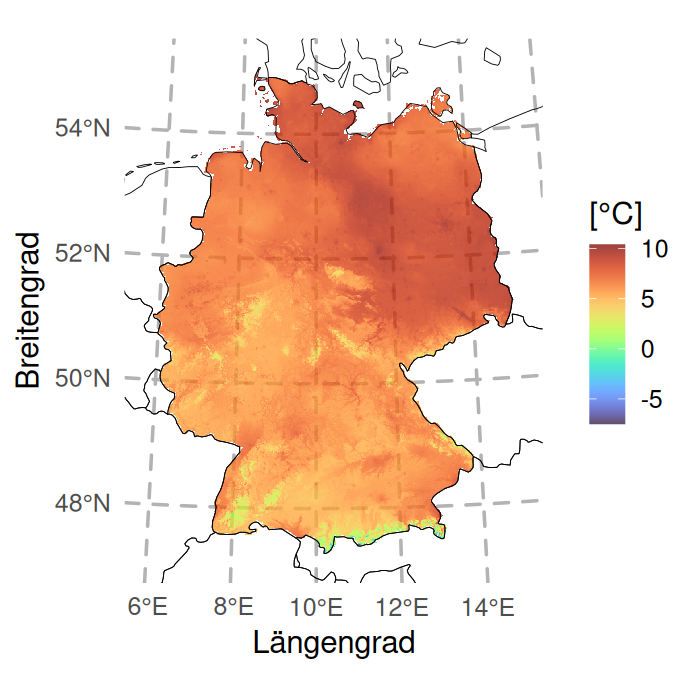
\includegraphics[width=0.55\linewidth]{figs/host_region_Rplot.png}
\caption{Modellgebiet HOSTRADA in EPSG:3034. Dargestellt ist die 2-m-Temperatur vom 3.11.2025 06:00 UTC.}
\label{fig:hostrada}
\end{figure}

\section{Projektion auf ein gemeinsames Gitter}\label{sec:proj}
Eine Besonderheit der ICON-Wettervorhersagemodelle ist das verwendete Gittersystem. Das Gitter des ICON-D2-EPS basiert auf einem unstrukturierten Dreiecksgitter in geografischen Koordinaten. Das Kürzel ICO im Modellnamen steht für \emph{ikosaedral}: Ein Ikosaeder ist ein zwanzigseitiges Polyeder. Dieses auf eine Kugel projiziert bildet die Grundlage des ICON Gitters. Die konkrete Gitterauflösung entsteht durch eine initiale Unterteilung in $n$ Root-Division-Schritte (R$n$) sowie anschließende $k$ Bisektionsschritte (B$k$), woraus ein R$n$B$k$-Gitter resultiert \parencite[Figure 2.1-2.3]{reinert2025icon_dwd}.

Im Gegensatz dazu liegen die HOSTRADA-Daten im projizierten Koordinatenreferenzsystem ETRS89 / LCC Europe (EPSG:3034) vor \parencite{dwd_hostrada_beschreibung}. Dieses basiert auf der Lambert-Conformal-Conic Projektion und ist für den europäischen Raum parametrisiert, sodass die Verzerrungen innerhalb Europas gering bleiben \parencite{map}. Vereinfacht wird bei der Projektion die Erdoberfläche zunächst auf einen Kegel abgebildet und anschließend in ein kartesisches Koordinatensystem überführt. Zudem ist das HOSTRADA feiner aufgelöst als das ICON-D2-EPS Gitter. Diesen Unterschied soll Abbildung \ref{fig:comparision} verdeutlichen.
\begin{figure}[h!]
\centering
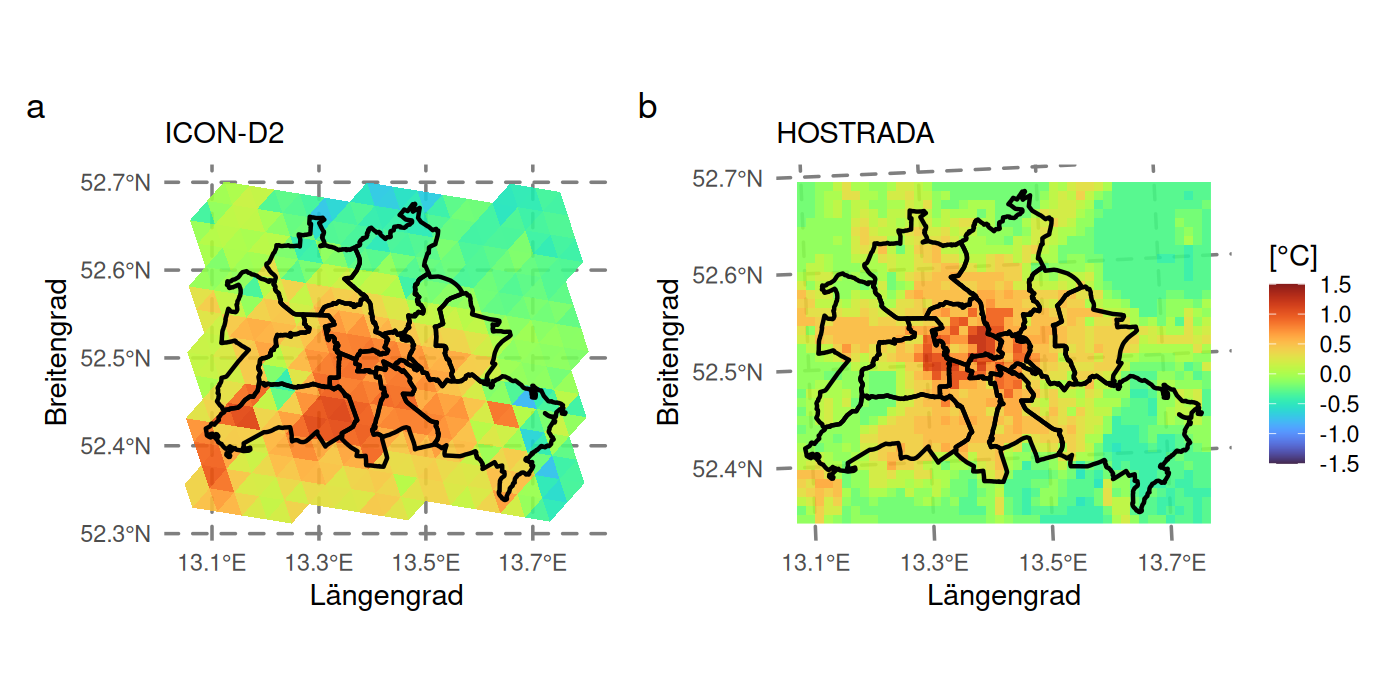
\includegraphics[width=\linewidth]{figs/proj_diff_Rplot.png}
\caption{ICON-D2-EPS Dreiecksgitter (a) im Vergleich zum HOSTRADA Raster (b) auf den Bereich Berlin eingegrenzt. Abgebildet ist die +24-h Vorhersage der 2-m-Temperatur des ersten Ensemblemitglieds zum 26.11.2025 00:00 UTC (a) und entsprechend die Temperatur vom 26.11.2025 00:00-UTC (b).}
\label{fig:comparision}
\end{figure}

Für einen Vergleich zwischen Modellvorhersagen und Beobachtungsdaten ist daher zunächst eine Überführung der beiden Modelle auf ein gemeinsames Koordinatensystem erforderlich. Wir projizieren hier die ICON-Daten auf das HOSTRADA-Gitter, das damit als Referenz für die Bewertung der Modellvorhersagen dient. Die Projektion auf das höher aufgelöste HOSTRADA-Gitter entspricht einem runterskalieren der Modellvorhersagen: Zwar werden die Modellfelder auf einer höheren räumlichen Auflösung dargestellt, der Informationsgehalt der Vorhersagen bleibt jedoch unverändert.

Ein wesentlicher praktischer Vorteil dieses Vorgehens besteht darin, dass das HOST\-RADA-Gitter von gängigen geostatistischen R-Paketen direkt verarbeitet werden kann, während das unstrukturierte Dreiecksgitter von ICON häufig nicht unterstützt wird.

Zur Änderung der Gitterprojektion empfiehlt der DWD die Nutzung des Kommandozeilenprogramms Climate Data Operators (CDO) \parencite{umwandlung}. CDO ist ein vom Max-Planck-Institut für Meteorologie entwickeltes Kommandozeilenprogramm zur Manipulation und Analyse von Klimadaten \parencite{CDO}. Für unstrukturierte Gitter wie das des ICON unterstützt CDO ausschließlich die Nearest-Neighbor-Interpolation. %Dies entspricht jedoch nicht dem Standardvorgehen des DWD, der abhängig von der jeweiligen Variable unterschiedliche Interpolationsverfahren einsetzt. So wird beispielsweise die 2-m-Temperatur mittels baryzentrischer Interpolation auf das Zielgitter übertragen \parencite{reinert2025icon_dwd}.

Nach der Projektion liegen somit sowohl die ICON-Vorhersagen als auch die HOST\-RADA-Beobachtungs\-daten auf dem gleichen räumlichen Gitter vor und können im weiteren Verlauf direkt miteinander verglichen und bewertet werden.


\section{Auswahl eines Datenausschnitts} \label{sec:used_data}
Für die Evaluation stehen mit den projizierten ICON-D2- und HOSTRADA-Daten umfangreiche, räumlich hochaufgelöste Daten für ganz Deutschland und verschiedene Zeiträume zur Verfügung. Für das das ICON-D2 existieren zudem verschiedene Vorhersagedurchläufe und Vorhersagehorizonte. Dadurch ergeben sich zahlreiche Möglichkeiten, Daten für eine Evaluation zusammenzustellen. Gegenstand der vorliegenden Arbeit sind Evaluationsmethoden probabilistischer Vorhersagen. Um diese gezielt zu untersuchen, grenzen wir die Daten ein, um eine überschaubare und nachvollziehbare Datengrundlage zu schaffen. Gleichzeitig soll die Auswahl realistische Bedingungen abbilden und nicht auf einen vollständig kontrollierten Anwendungsfall beschränkt sein. Wir schränken die Datenmenge hinsichtlich des betrachteten Zeitraums, des Vorhersagegebiets, des Vorhersagedurchlaufs und der Vorhersagehorizonte ein.

Als Evaluationszeitraum betrachten wir den November 2025. Die Beschränkung auf einen Monat ermöglicht eine überschaubare Auswertung.  Neben Evaluationsdaten verwenden wir unter anderem statistisches Postprocessing, um aus den rohen Ensemblevorhersagen des DWD probabilistische Vorhersagen zu erstellen. Dazu bedarf es Trainingsdaten, üblich ist hierbei ein Trainingsfenster von 20 bis 40 Tagen \parencite{gneiting2014calibration}, sodass Vorhersage und Verifikationsdaten des Oktobers 2025 ebenfalls als Daten einfließen.

Das Untersuchungsgebiet wird auf eine Region um Berlin eingegrenzt. Die Wahl der Region erfolgte in Abstimmung mit dem Betreuer sowohl aufgrund eines persönlichen Bezugs zur Region als auch aufgrund ihrer hohen Bevölkerungsdichte und der damit verbundenen gesellschaftlichen Relevanz. Als Grundlage für die probabilistischen Vorhersagen dienen die stündlichen Ensemblevorhersagen des ICON-D2-EPS. Dabei betrachten wir jeweils den um 00:00 UTC initialisierten Modelllauf. Dies stellt eine einfache und nachvollziehbare Auswahl des Modelllaufs dar, weil dieser der erste verfügbare Modelllauf des jeweiligen Tages ist. Analysiert werden die Vorhersagehorizonte von 24 und 48 Stunden. Die beiden Horizonte wählen wir, weil zwischen ihnen 24 Stunden liegen und wir somit für beide Horizonte dieselben Beobachtungsdaten des Novembers verwenden können. Dadurch lassen sich die Vorhersagehorizonte direkt miteinander vergleichen.

Der Auswahl der Daten entsprechend sind die Ergebnisse also als exemplarische Untersuchung probabilistischer Vorhersagen zu verstehen und nicht als vollständige oder repräsentative Evaluation der Vorhersagequalität des ICON-D2-EPS.


\section{Vorbereitung der Daten} 
Die Vorbereitung der Vorhersagedaten folgende Schritte: Mithilfe des CDO-Befehls \texttt{gennn} wurden zunächst Interpolationsgewichte auf Basis der Gitterbeschreibungen von HOSTRADA und ICON-D2-EPS erzeugt und als NetCDF-Datei gespeichert. Anschließend wurden über das Webinterface von PAMORE die ICON-D2-EPS-Daten für den Zeitraum vom 1. Oktober 2025 bis zum 30. November 2025 jeweils täglich um 00:00 UTC mit Vorhersagehorizonten von 24 und 48 Stunden abgefragt. Die Daten wurden anschließend über den FTP-Server heruntergeladen und gespeichert. Mithilfe der zuvor erzeugten Interpolationsgewichte wurden die ICON-D2-EPS Daten für jeden Vorhersagehorizont mit dem CDO-Befehl \texttt{remap} auf das HOSTRADA-Gitter projiziert. Abschließend wurden die Ensemblemitglieder je Vorhersagehorizont und Tag zu einer gemeinsamen Datei zusammengeführt und als NetCDF-Datei gespeichert. Dieser gesamte Prozess wurde mithilfe eines Python Skripts teilweise automatisiert. Die HOSTRADA-Daten mussten nicht weiter vorverarbeitet werden.

\section{Zusammenfassung und Indizierung} \label{sec:indx}

Zusammenfassend vergleichen wir probabilistische Vorhersagen, die aus den auf das HOSTRADA-Gitter projizierten Ensemblemitgliedern des ICON-D2-EPS des jeweils um 00:00 UTC initialisierten Modelllaufs abgeleitet werden, mit den entsprechenden Temperaturbeobachtungen des HOSTRADA. Der Untersuchungszeitraum umfasst den November 2025 und damit insgesamt 30 Tage vom 01.11.2025, 00:00 UTC, bis zum 30.11.2025, 00:00 UTC. Analysiert werden Vorhersagehorizonte von 24 und 48 Stunden für ein Vorhersagegebiet um Berlin, das insgesamt $38 \times 46 = 1748$ Gitterzellen umfasst.

Zur einheitlichen Beschreibung der Verifikationsdaten führen wir folgende Indizierung ein: Es bezeichne $t \in T = \{1,\dots,30\}$ den Verifikationstag im November 2025, \mbox{$l \in L = \{1,\dots,1748\}$} die jeweilige Gitterzelle, $m \in M = \{1,\dots,20\}$ das Ensemblemitglied des ICON-D2-EPS sowie $h \in H = \{24\h, 48\h\}$ den betrachteten Vorhersagehorizont. 

Wir schreiben also $y_{l}^{(t)}$ für die beobachtete HOSTRADA Temperatur zum Zeitpunkt 00:00 UTC am Verifikationstag $t$ in der Gitterzelle $l$. Entsprechend schreiben wir  $x_{l,h,m}^{(t)}$ für die Punktvorhersage für 00:00 UTC zum Verifikationstag $t$ an Gitterzelle $l$, erzeugt vom $m$-ten Ensemblemitglied zum Vorhersagehorizont $h$. Initialisiert ist diese Vorhersage entweder einen Tag ($h=24\h$) oder zwei Tage ($h=48\h$) vor dem Verifikationstag. Die Temperatur geben wir in Grad Celsius an. Zur Veranschaulichung der Struktur und Beschaffenheit der Verifikationsdaten betrachten wir exemplarisch den Vorhersagehorizont $h=24\h$. Tabelle \ref{tab:datensatz} zeigt hierzu einen beispielhaften Datenausschnitt, während Abbildung \ref{fig:daten_schema} die Daten schematisch darstellt.

\begin{table}[ht]
    \centering
    \fontsize{10.5}{12}\selectfont
    \newcolumntype{C}{>{\centering\arraybackslash}X}
    \newcolumntype{Y}{>{\centering\arraybackslash}p{2cm}}
    \caption{Ausschnitt zum Aufbau des Verifikationsdatensatzes zum Vorhersagehorizont $24\h$.}
    \label{tab:datensatz}
    \begin{tabularx}{\textwidth}{Y C C C C C C C C}
        \toprule
        Datum & $t$ & $l$ & $y_{l}^{(t)}$ & $x_{l,24\h,1}^{(t)}$ & $x_{l,24\h,2}^{(t)}$ & $x_{l,24\h,3}^{(t)}$ & $\dots$ & $x_{l,24\h,20}^{(t)}$ \\
        \midrule
        2025110100 & 1 & 1 & 7.3 & 7.5 & 7.9 & 6.2 & $\dots$ & 7.5 \\
        2025110100 & 1 & 2 & 7.3 & 7.4 & 7.9 & 6.3 & $\dots$ & 7.4 \\
        2025110100 & 1 & 3 & 7.3 & 7.5 & 8.0 & 6.5 & $\dots$ & 7.4 \\
        2025110100 & 1 & 4 & 7.4 & 7.5 & 8.0 & 6.5 & $\dots$ & 7.4 \\
        2025110100 & 1 & 5 & 7.7 & 7.7 & 8.2 & 6.8 & $\dots$ & 7.6 \\
        $\vdots$ & $\vdots$ & $\vdots$ & $\vdots$ & $\vdots$ & $\vdots$ & $\vdots$ & $\vdots$ & $\vdots$ \\
        2025113000 & 30 & 1744 & 4.7 & 2.7 & 4.1 & 2.7 & $\dots$ & 4.8 \\
        2025113000 & 30 & 1745 & 4.7 & 2.5 & 4.0 & 2.6 & $\dots$ & 4.7 \\
        2025113000 & 30 & 1746 & 4.7 & 2.4 & 3.7 & 2.3 & $\dots$ & 4.7 \\
        2025113000 & 30 & 1747 & 4.7 & 2.4 & 3.7 & 2.3 & $\dots$ & 4.7 \\
        2025113000 & 30 & 1748 & 4.7 & 2.2 & 3.5 & 2.2 & $\dots$ & 4.8 \\
        \bottomrule
    \end{tabularx}
\end{table}


\begin{figure}[h] 
\centering
\resizebox{.85\textwidth}{!}{
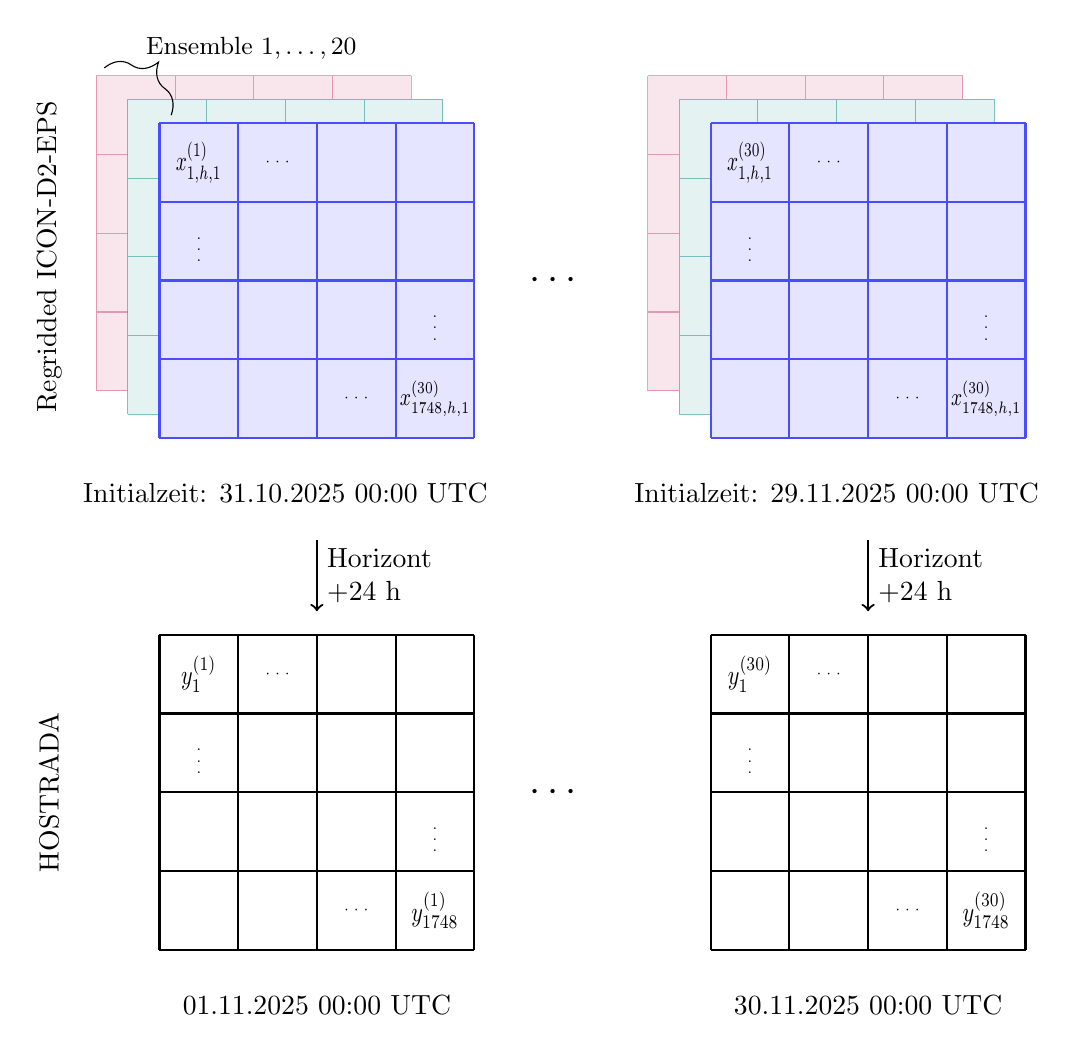
\begin{tikzpicture}%[scale=0.5,, transform shape]
\def\N{4}
\def\dy{-6.5} % vertikaler Versatz der Verifikationszeile nach unten
\def\dx{7} %horizontaler versatz der gitter

% =========================================================
% Zeilenbeschriftung links: Ensemble-Reihe
% =========================================================
\node[rotate=90] at (-1.4,2.3) {Regridded ICON-D2-EPS};
% =========================================================
% ENSEMBLE-REIHE (oben)
% =========================================================
% --- Ensemble-Grafik 1 ---
\begin{scope}[shift={(0,0)}]
% Ensemble 3 (hinten)
\begin{scope}[shift={(-0.8,0.6)}]
    \fill[purple!10] (0,0) rectangle (\N,\N);
    \draw[purple!70, opacity=0.5] (0,0) grid (\N,\N);
\end{scope}
% Ensemble 2 (mittig)
\begin{scope}[shift={(-0.4,0.3)}]
    \fill[teal!10] (0,0) rectangle (\N,\N);
    \draw[teal!70, opacity=0.7] (0,0) grid (\N,\N);
\end{scope}
% Ensemble 1 (vorne)
\fill[blue!10] (0,0) rectangle (\N,\N);
\draw[blue!70, thick] (0,0) grid (\N,\N);


% Werte
\node  at (0.5,\N-0.5) { \scalebox{0.7}[1]{$x_{1,h,1}^{(1)}$}};
\node[font=\small] at (\N-0.5,0.5) {\scalebox{0.77}[1]{$x_{1748,h,1}^{(30)}$}};
% rechts daneben
\node[font=\tiny] at (1.5,\N-0.5) {$\cdots$};
% darunter
\node[font=\tiny] at (0.5,\N-1.5) {$\vdots$};
% links neben B
\node[font=\tiny] at (\N-1.5,0.5) {$\cdots$};
% oberhalb von B
\node[font=\tiny] at (\N-0.5,1.5) {$\vdots$};


% Klammer
\draw[decorate, decoration={brace, amplitude=13pt}]
(-0.7,\N+.7) -- (0.15,\N+.1)
node[near end, yshift=20pt,xshift=35pt,font=\small]
{Ensemble $1, \ldots, 20$};
\node at (1.6,-0.7) {Initialzeit: 31.10.2025 00:00 UTC};
\end{scope}

\node at (5,2) {\Large $\cdots$};

% --- Ensemble-Grafik 2 ---
\begin{scope}[shift={(\dx,0)}]
\begin{scope}[shift={(-0.8,0.6)}]
    \fill[purple!10] (0,0) rectangle (\N,\N);
    \draw[purple!70, opacity=0.5] (0,0) grid (\N,\N);
\end{scope}
\begin{scope}[shift={(-0.4,0.3)}]
    \fill[teal!10] (0,0) rectangle (\N,\N);
    \draw[teal!70, opacity=0.7] (0,0) grid (\N,\N);
\end{scope}
\fill[blue!10] (0,0) rectangle (\N,\N);
\draw[blue!70, thick] (0,0) grid (\N,\N);
\node at (1.6,-0.7) {Initialzeit: 29.11.2025 00:00 UTC};


\node  at (0.5,\N-0.5) { \scalebox{0.7}[1]{$x_{1,h,1}^{(30)}$}};
\node[font=\small] at (\N-0.5,0.5) {\scalebox{0.77}[1]{$x_{1748,h,1}^{(30)}$}};
% rechts daneben
\node[font=\tiny] at (1.5,\N-0.5) {$\cdots$};
% darunter
\node[font=\tiny] at (0.5,\N-1.5) {$\vdots$};
% links neben B
\node[font=\tiny] at (\N-1.5,0.5) {$\cdots$};
% oberhalb von B
\node[font=\tiny] at (\N-0.5,1.5) {$\vdots$};
\end{scope}

% =========================================================
% Pfeil: Vorhersagehorizont (nach unten, innerhalb der Spalte)
% =========================================================
\draw[->, thick]
    (2,-1.3) -- node[right, align=left] {Horizont\\ +24 h} (2,\dy+\N+0.3);
\draw[->, thick]
    (2+\dx,-1.3) -- node[right, align=left] {Horizont\\ +24 h} (2+\dx,\dy+\N+0.3);
% =========================================================
% Zeilenbeschriftung links: Verifikations-Reihe
% =========================================================
\node[rotate=90] at (-1.4,\dy+2) {HOSTRADA};

% =========================================================
% VERIFIKATIONS-REIHE (unten)
% =========================================================
\begin{scope}[shift={(0,\dy)}]
\draw[black, thick] (0,0) grid (\N,\N);
\node at (2,-0.7) {01.11.2025 00:00 UTC};

\node  at (0.5,\N-0.5) { \scalebox{0.8}[1]{$y_{1}^{(1)}$}};
\node at (\N-0.5,0.5) {\scalebox{0.8}[1]{$y_{1748}^{(1)}$}};
\node[font=\tiny] at (1.5,\N-0.5) {$\cdots$};
\node[font=\tiny] at (0.5,\N-1.5) {$\vdots$};
\node[font=\tiny] at (\N-1.5,0.5) {$\cdots$};
\node[font=\tiny] at (\N-0.5,1.5) {$\vdots$};

\end{scope}

\node at (5,\dy+2) {\Large $\cdots$};


\begin{scope}[shift={(7,\dy)}]
\draw[black, thick] (0,0) grid (\N,\N);
\node at (2,-0.7) {30.11.2025 00:00 UTC};
\node  at (0.5,\N-0.5) { \scalebox{0.8}[1]{$y_{1}^{(30)}$}};
\node at (\N-0.5,0.5) {\scalebox{0.8}[1]{$y_{1748}^{(30)}$}};
\node[font=\tiny] at (1.5,\N-0.5) {$\cdots$};
\node[font=\tiny] at (0.5,\N-1.5) {$\vdots$};
\node[font=\tiny] at (\N-1.5,0.5) {$\cdots$};
\node[font=\tiny] at (\N-0.5,1.5) {$\vdots$};
\end{scope}

\end{tikzpicture}
}
\caption{Schematische Darstellung der Verifikationsdatenpaare zum Vorhersagehorizont $h=24\h$.}
\label{fig:daten_schema}
\end{figure}

\FloatBarrier
\section{Deskription der Daten} \label{sec:desc}
\subsection{HOSTRADA Temperaturbeobachtungen November 2025}
Wir betrachten zunächst die zeitlichen und anschließend die räumlichen Aspekte der Temperaturbeobachtungen anhand visueller Darstellungen. Abbildung \ref{fig:nov_temp} zeigt die zeitliche Entwicklung und Häufigkeitsverteilung der Temperaturen Berlins für den November 2025, 00:00 UTC der HOSTRADA-Verifikationsdaten. Die zeitliche Entwicklung der Temperaturen beginnt mit einer Abkühlung vom Monatsbeginn bis zum letzten Monatsdrittel. Die niedrigsten Temperaturen werden zwischen dem 21. und 24. November erreicht. Anschließend steigen die Temperaturen zum Monatsende wieder leicht an. Zudem ist erkennbar, dass die Gesamtvariabilität der Temperaturbeobachtungen überwiegend auf zeitlichen Unterschieden zwischen den Tagen beruht. Innerhalb eines Tages ist die Variation oft gering.

\begin{figure}[h]
    \centering
    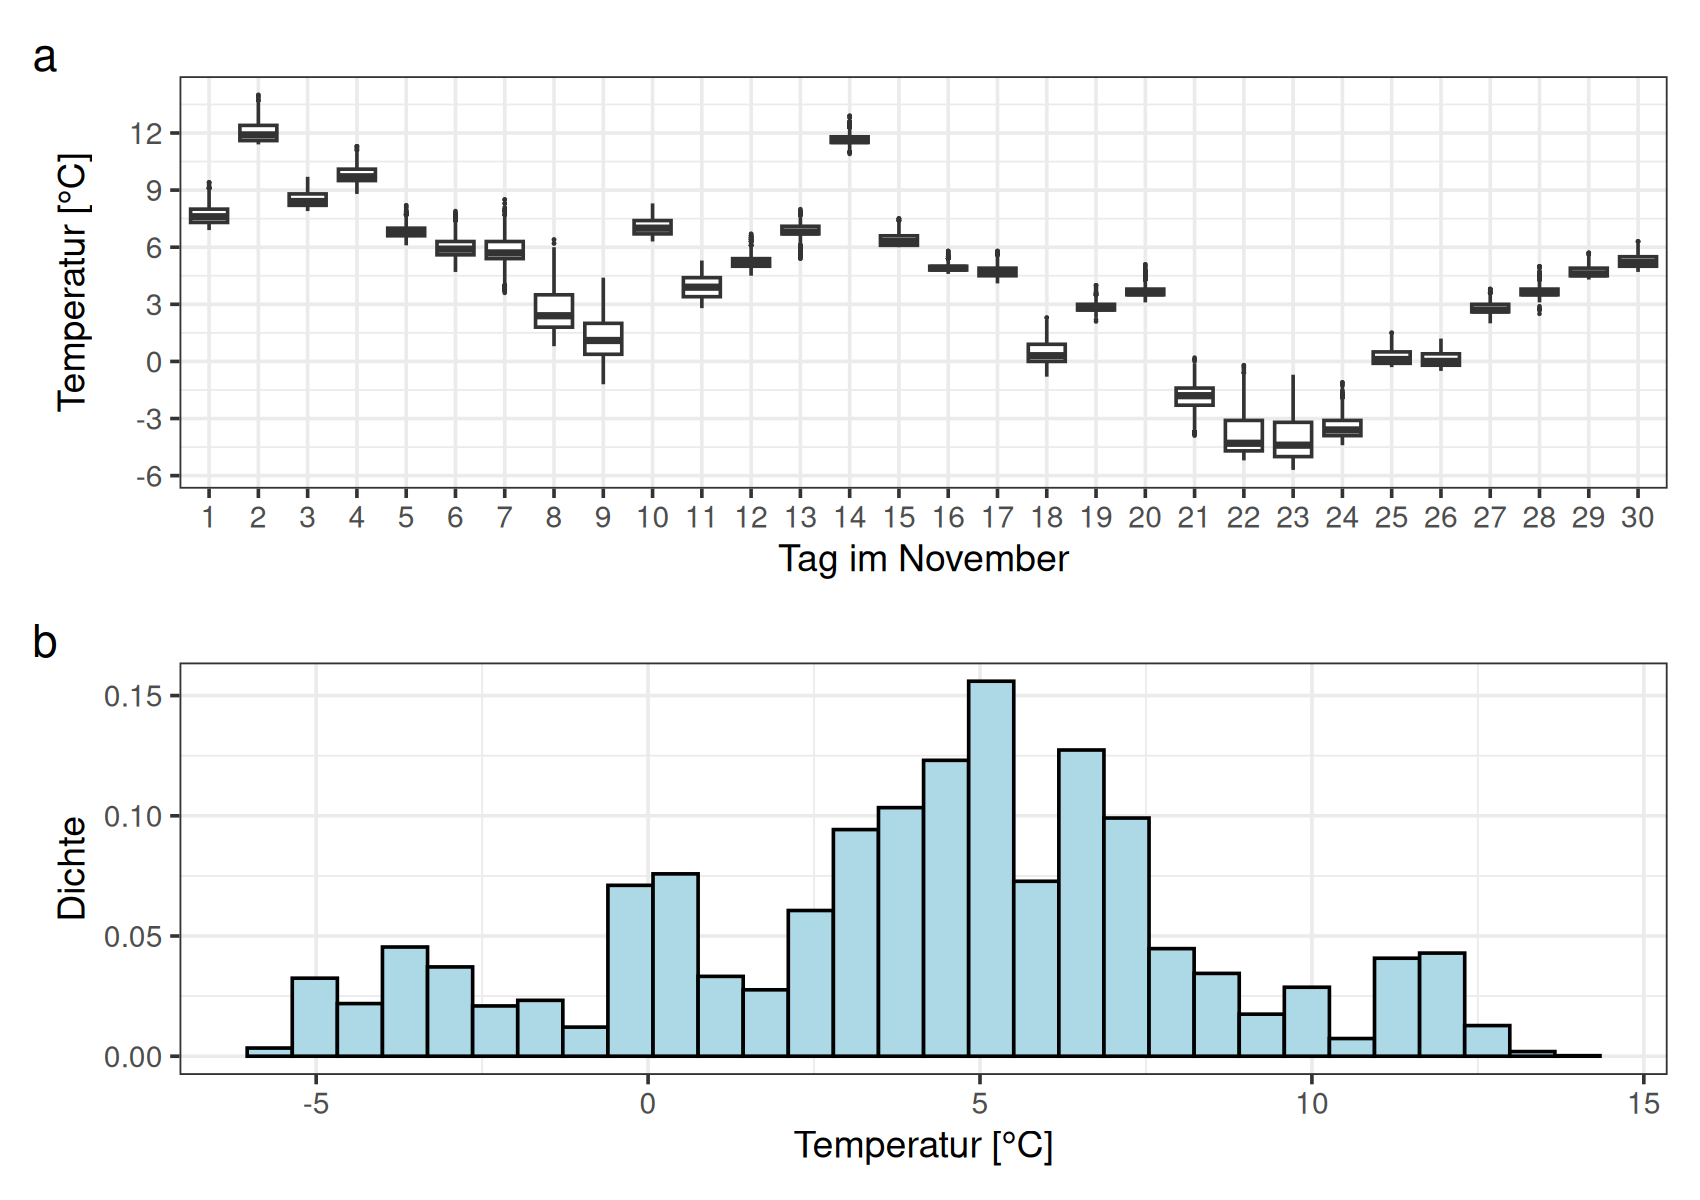
\includegraphics[width=0.9\linewidth]{figs/nov_desc.png}
    \caption{HOSTRADA: Temperatur in Berlin im November 2025, 00:00 UTC. Boxplots der Temperaturverteilung pro Tag über alle Gitterzellen (a) und Histogramm der beobachteten Temperaturen über alle Tage und Gitterzellen (b).}
    \label{fig:nov_temp}
\end{figure}

Die Häufigkeitsverteilung weißt einen Schwerpunkt zwischen etwa $4\C$ und $6\C$ auf. Temperaturen unter dem Gefrierpunkt sowie Werte oberhalb von $10\C$ treten selten auf. Die Verteilung ist asymmetrisch, ungleichmäßig und es zeigen sich mehrere lokale Häufigkeitsmaxima. Diese spiegeln sowohl die milde Witterung zu Monatsbeginn als auch die Kältephase vom 21. bis 24. wider.

Abbildung \ref{fig:nov_temp_spat} zeigt die räumliche Verteilung der mittleren Temperatur im November 2025 um  00:00 UTC über das Untersuchungsgebiet.
Dabei wird  ein Stadt-Land-Gradient deutlich: Die höchsten Temperaturen werden im Innenstadtbereich Berlins erreicht und an den Randgebieten nehmen die Temperaturen kontinuierlich ab. Besonders die südöstlichen und nordöstlichen Stadtränder weisen vergleichsweise niedrige Temperaturen auf. Dieses räumliche Muster entspricht einem Urban-Heat-Island-Effekt, der im HOSTRADA explizit modelliert wird und daher erwartungsgemäß erkennbar ist \parencite{krahenmann_high-resolution_2018}.

Ergänzend dazu können wir ausgewählte räumliche Eigenschaften des Untersuchungsgebiets genauer betrachten. Dazu ist in Abbildung \ref{fig:berlin_spat} die Verteilung von Gewässern, Wald- und Ackerflächen im untersuchten Gebiet dargestellt. Anhand dieser Abbildung wird deutlich, dass in der HOSTRADA Temperaturkarte (vgl. Abbildung \ref{fig:nov_temp_spat}) Wälder und Ackerflächen geringere mittlere Temperaturen als andere Bereiche aufweisen. Gewässer fallen hingegen nicht besonders auf.

\begin{figure}[h]
    \centering
    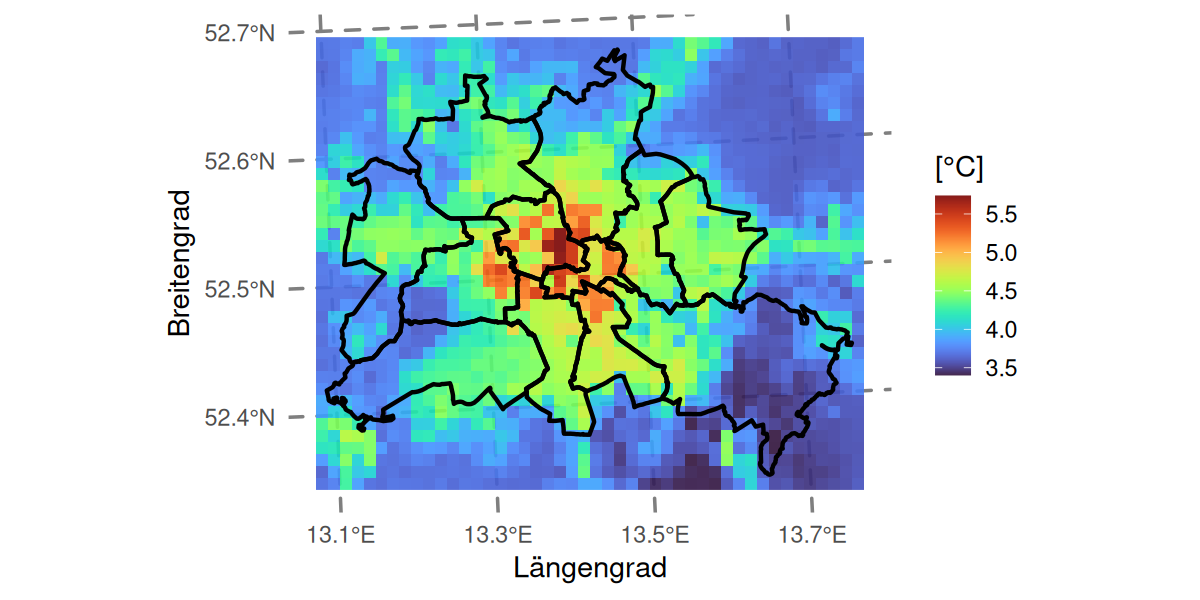
\includegraphics[width=\linewidth]{figs/nov_spat_Rplot.png}
    \caption{HOSTRADA: Mittlere Temperatur in Berlin im November 2025, 00:00 UTC pro Gitterzelle.}
    \label{fig:nov_temp_spat}
\end{figure}



\begin{figure}[h]
    \centering
    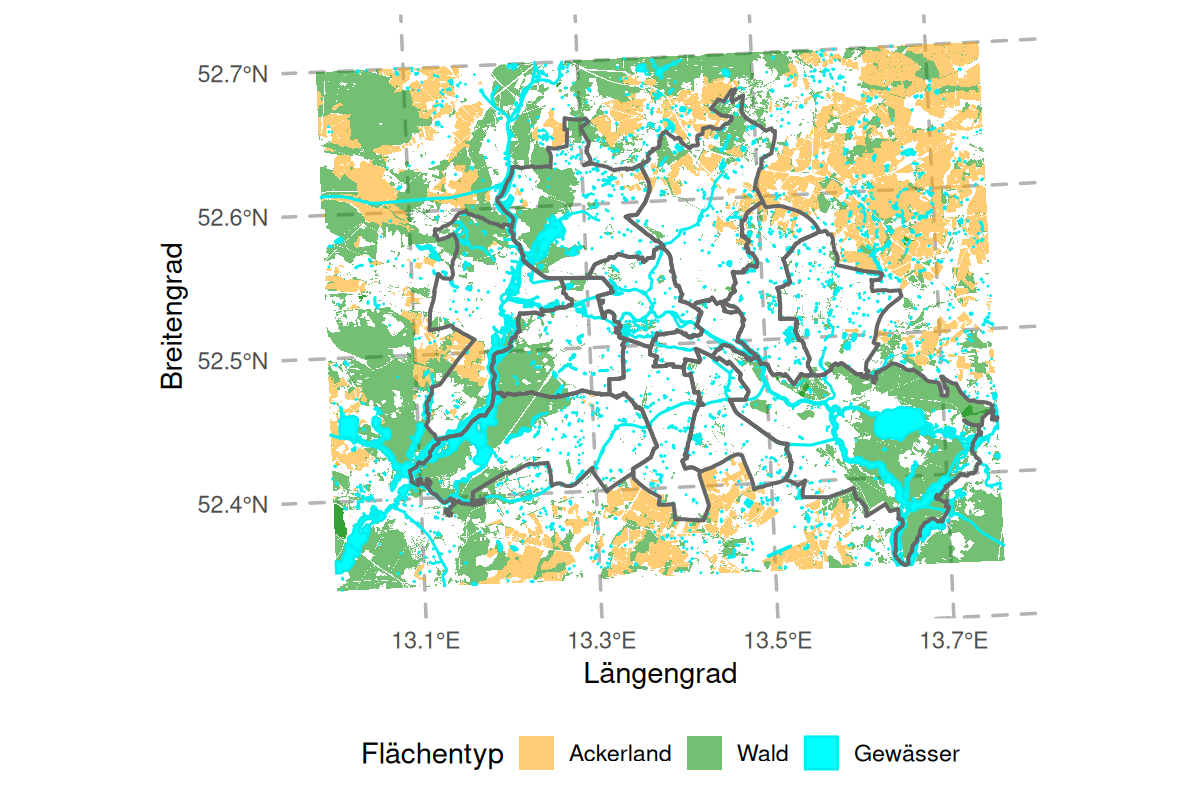
\includegraphics[width=.9\linewidth]{figs/berlin_geo_Rplot.png}
    \caption{Räumliche Verteilung der Gewässer, Wald- und Ackerflächen im untersuchten Gebiet.
    Datengrundlage: \href{https://download.geofabrik.de/europe/germany/brandenburg.html}{OpenStreetMap-Daten}.}
    \label{fig:berlin_spat}
\end{figure}


\FloatBarrier
\subsection{ICON-D2-EPS Temperaturvorhersagen November 2025}
Um die ICON-D2-EPS-Vorhersagen zu beschreiben, vergleichen wir sie direkt mit den HOSTRADA-Daten. Dabei betrachten wir, wie im vorherigen Abschnitt, zunächst zeitliche und anschließend räumliche Aspekte.

Abbildung \ref{fig:icon_time} zeigt die zeitliche Entwicklung der ICON-D2-Ensemblevorhersagen im Vergleich zur HOSTRADA. Insgesamt bilden die Ensemblevorhersagen den zeitlichen Temperaturverlauf der HOSTRADA-Daten gut ab. Beim höheren Vorhersagehorizont nimmt die Streuung der Ensemblemitglieder jedoch zu. Auffällig ist zudem eine tendenzielle Überschätzung der Temperaturen um den 9.11 sowie dem 22.11. Dabei zeichnet sich jedoch kein Ensemblemitglied durch eine auffallend systematisch zu hohe oder zu niedrige Temperaturvorhersage aus.

Abbildung \ref{fig:nov_temp_spat} zeigt die räumliche Verteilung der mittleren Temperaturvorhersagen über alle Ensemble getrennt nach Vorhersagehorizont. Die räumliche Struktur erscheint dabei unabhängig vom Vorhersagehorizont. Wie bei den HOSTRADA-Daten wird ein Stadt-Land-Gradient deutlich. Die Darstellung ist jedoch insgesamt glatter und im Stadtkern weniger extrem. Im Vergleich zu den HOSTRADA-Daten (Abbildung \ref{fig:nov_temp_spat}) fallen jedoch die Gewässer Teglersee (links oben), Havel (links unten) und insbesondere der Große Müggelsee (rechts unten) (vgl. Abbildung \ref{fig:berlin_spat}) durch eine höhere Temperatur als deren Umgebung auf.






\begin{figure}[h]
    \centering
    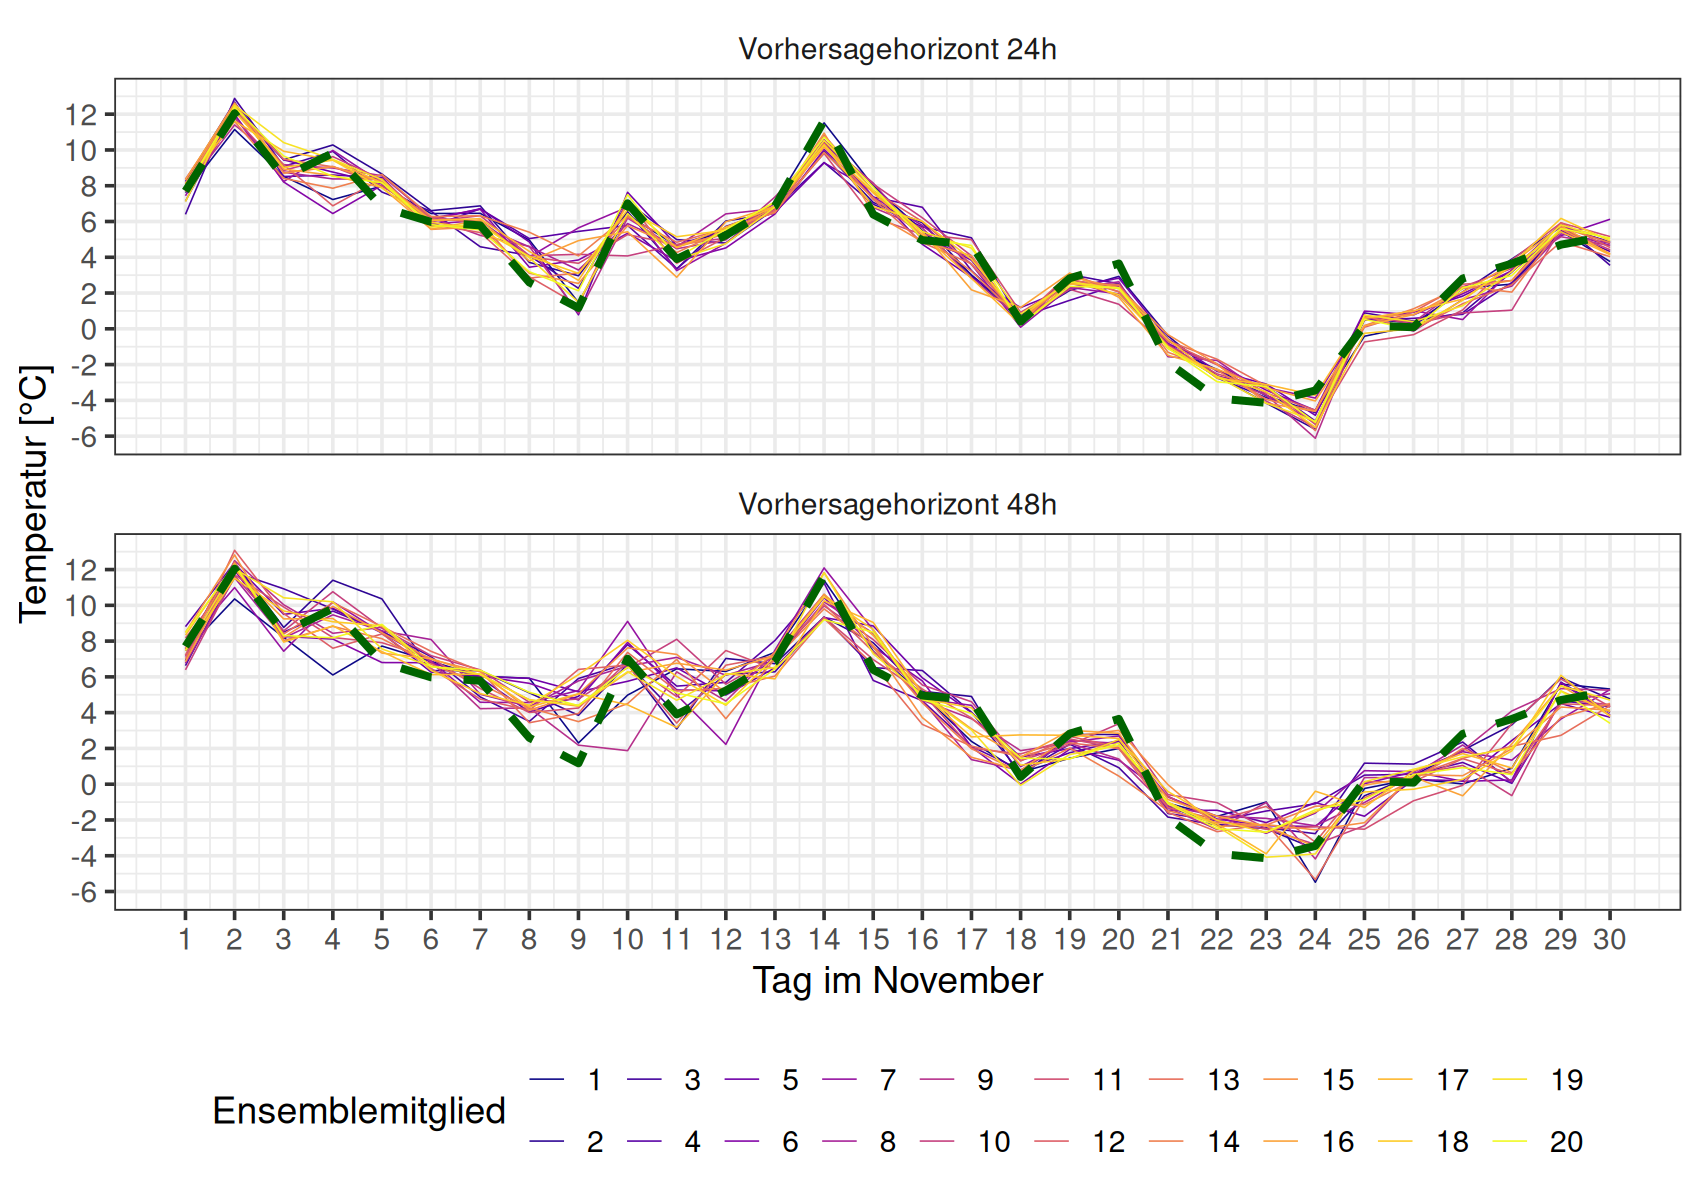
\includegraphics[width=.95\linewidth]{figs/icon_time.png}
    \caption{ICON-D2-EPS: Mittlere Temperatur in Berlin pro Tag im November 2025, 00:00 UTC pro Ensemblemitglied für beide Vorhersagehorizonte. Die gestrichelte Linie zeigt die HOSTRADA- Temperatur als Referenz.}
    \label{fig:icon_time}
\end{figure}

\begin{figure}[!ht]
    \centering
    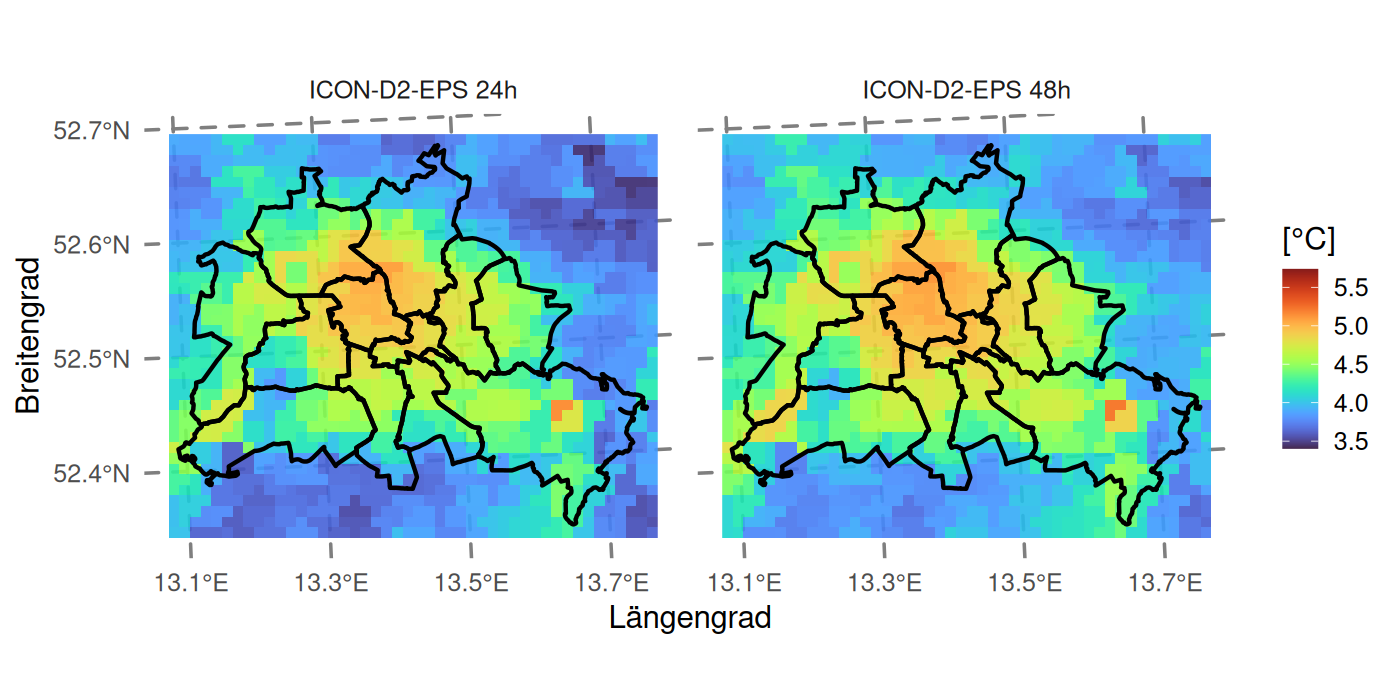
\includegraphics[width=1.02\linewidth]{figs/mean_icon_spat_Rplot.png}
    \caption{
     ICON-D2-EPS: Mittlere Temperatur in Berlin pro Gitterzelle im November 2025, 00:00 UTC getrennt nach Vorhersagehorizont, über alle Ensemblemitglieder gemittelt.}
    \label{fig:icon_temp_spat}
\end{figure}





\chapter{Vorhersagen und Evaluationsvorgehen} \label{chap:meth}
Im vorherigen Kapitel haben wir die Datengrundlage beschrieben. Für die Evaluation fehlen jedoch noch probabilistische Vorhersagen. In diesem Kapitel soll es daher vornehmlich darum gehen, wie wir auf der Basis von Ensemblevorhersagen probabilistische Vorhersagen erstellen können. Zu Beginn beschreiben wir jedoch in Abschnitt \ref{sec:sofware} die verwendete Software für die Berechnungen in der vorliegenden Arbeit. Erst dann gehen wir in den Abschnitten \ref{sec:pre_postproc} und \ref{sec:postproc} darauf ein, wie wir die probabilistischen Vorhersagen erstellen. Schließlich fassen wir in Abschnitt \ref{sec:meth_eval} die zur Evaluation erstellten Vorhersagen zusammen und erläutern kurz das Evaluationsvorgehen. Abschließend formulieren wir einige Erwartungen an die Güte der erstellten Vorhersagen.

\section{Software, Implementierung und Reproduzierbarkeit} \label{sec:sofware}
Für das Erstellen der probabilistischen Vorhersagen, die Evaluation sowie den theoretischen Teil dieser Arbeit wurden alle Analysen mit \texttt{RStudio} \parencite{Rstudio} in der Programmiersprache R \parencite{R} durchgeführt. Im Folgenden werden die wichtigsten der verwendeten Pakete vorgestellt. Zur Bearbeitung der Daten wurde das Paket \texttt{tidyverse} \parencite{tidy} verwendet. Insbesondere die darin enthaltene Bibliothek \texttt{ggplot2} \parencite{ggplot2} bildet die Grundlage für alle in dieser Arbeit erstellten Abbildungen. Für die Bearbeitung und Darstellung geografischer Daten kamen die Pakete \texttt{terra} \parencite{terra}, \texttt{tidyterra} \parencite{tidyterra} und \texttt{sf} \parencite{sf} zum Einsatz. Die Regressionen im Rahmen des Postprocessings wurden mit dem Paket \texttt{crch} \parencite{crch} durchgeführt. Zur Berechnung des Quantilscores und des CRPS kam das Paket \texttt{scoringRules} \parencite{scoringRules} zum Einsatz. Der PAV-Algorithmus wurde mit dem Paket \texttt{isotone} \parencite{isotone} berechnet. 

Für die im Rahmen der Evaluation verwendeten Methoden war kein R-Paket bekannt, das alle benötigten Funktionalitäten bereitstellt. Die Implementierung greift jedoch teilweise auf bereits vorhandenen Code zurück. So wurde der Code zur Erstellung der Reliabilitätsdiagramme auf Grundlage des ergänzenden Materials \textcite{gneiting2023supp} angepasst und unter anderem auf \texttt{ggplot2} umgestellt. In ähnlicher Weise basiert die Implementierung der Zerlegungsdiagramme auf dem Code Material von \textcite{gneiting2023model}. Für die Zerlegung des CRPS mithilfe des Quantilscores lag hingegen kein entsprechender Beispielcode vor, sodass diese Methode selbst implementiert wurde. Der vollständige Code zur Auswertung ist in einem GitHub-Repository über
\begin{quote}
    \url{https://github.com/harro-rejewski/bachelor_thesis.git}
\end{quote}
verfügbar. Zur Gewährleistung der Reproduzierbarkeit können entweder das bereitgestellte Docker-Image oder die entsprechende \texttt{.lock}-Datei verwendet werden, über die sich die verwendeten Paketversionen nachvollziehen und reproduzieren lassen.


\section{Erstellen von probabilistischen Vorhersagen}\label{sec:pre_postproc}
Gegeben seien die Ensemblevorhersagen für einen Verifikationstag, Ort und Vorhersagehorizont
\[
x_{l,h}^{(t)}=\left(x_{l,h,1}^{(t)},\dots,x_{l,h,20}^{(t)}\right).
\]
Ziel ist es, auf Basis dieser Information eine probabilistische Vorhersage zu erstellen. Formal suchen wir also eine Abbildung, die die Ensemblevorhersagen in eine Wahrscheinlichkeitsverteilung und damit in eine Vorhersage $F^{(t)}_{l,h}$ überführt\footnote{Im Sinne des Vorhersageraums \ref{def::room} entspricht dies also einem Markovkern.}, wobei $F_{l,h}^{(t)}$ die probabilistische Vorhersage für die Gitterzelle $l$, den Vorhersagehorizont $h$ und den Verifikationstag $t$ bezeichnet. Idealerweise approximiert diese Vorhersage die bedingte Verteilung, wodurch die Eigenschaft der Auto-Kalibrierung aus Abschnitt \ref{sec:auto_cal} erfüllt wäre.
\[
F^{(t)}_{l,h}(y) \approx \mathbb{P}(Y^{(t)}_{l}\le y \mid X_{l,h}^{(t)}=x^{(t)}_{l,h})\,,
\]
wobei $X_{l,h}^{(t)}$ die Zufallsvariable der Ensemblevorhersagen, und  $Y^{(t)}_{l}$ die der Temperaturbeobachtung zugrundeliegende Zufallsvariable bezeichnen. Wir fassen also sowohl die Ensemblevorhersagen $x_{l,h}^{(t)}$ als auch die Temperaturbeobachtung $y^{(t)}_{l}$ als Realisationen von Zufallsvariablen auf. 

Die einfachste probabilistische Vorhersage, die wir nun erstellen können, ist die empirische Verteilung der Ensemblemitglieder. Dem Ensemble ordnen wir also die Verteilungsfunktion
\[
F_{l,h}^{(\mathrm{emp},t)}(y)= \frac{1}{20}\sum_{m=1}^{20} \mathds{1}\!\left\{x_{l,h,m}^{(t)}\le y\right\}
\]
zu. Wir nennen diese Vorhersage die \emph{empirische Vorhersage}.


\section{Statistisches Postprocessing}\label{sec:postproc}
Ensemblevorhersagen weisen häufig systematische Fehler in Form von Bias und Dispersionsfehlern auf \parencite{vannitsem_statistical_2021}. Dispersionsfehler äußern sich meist in einer zu geringen Streuung der Ensemblemitglieder. Aufgrund dieser möglichen Fehler ist es sinnvoll, Ensemblevorhersagen mithilfe statistischer Postprocessing Verfahren nachzubearbeiten und nicht direkt die empirische Verteilung dieser als Vorhersage zu verwenden \parencite{vannitsem_statistical_2021, gneiting2014probabilistic}.

Die Variante des Postprocessings, die wir anwenden, ist ein univariater Ansatz. Dabei erhalten wir für jede Kombination aus Gitterzelle und Vorhersagehorizont eine separate Vorhersage \parencite{climaguidelines}. Räumliche und zeitliche Abhängigkeiten bleiben somit nur durch die Ensemblesvorhersagen erhalten und werden im Postprocessing nicht explizit modelliert. Dies steht im Gegensatz zu Ansätzen, bei denen ein gemeinsames multivariates Modell über mehrere Orte oder Zeitpunkte spezifiziert wird \parencite{vannitsem_statistical_2021}.

Konkret nutzten wir hier  \emph{Ensemble Model Output Statistics} (EMOS). Hierbei handelt es sich, um eine verbreitete univariate Postprocessing-Methode \parencite{gneiting2005emos,gebetsberger2018estimation}. Dabei dienen die Ensemblemitglieder als Kovariaten einer verteilungsbasierten parametrischen Regression, deren Parameter mithilfe von Trainingsdaten geschätzt werden. Seinen dazu vereinfacht ohne Zelle und Horizont  $x_1,\dotsc,x_M$ Ensemblevorhersagen und $Y$ der Vorhersagegegenstand und $f$ eine zu spezifizierende parametrische Wahrscheinlichkeitsverteilung. Dann lautet das allgemeine EMOS Modell
\[
Y \mid x_1,\dotsc,x_M \sim f(\,\cdot \mid x_1,\dotsc,x_M\,).
\]

Betrachten wir die Temperatur als Response, so wird diese im Rahmen von EMOS häufig durch eine Normalverteilung modelliert, wobei die Ensemblemitglieder als austauschbar gelten \parencite{gneiting2014probabilistic}. In diesem Fall entspricht EMOS einer heteroskedastischen Gaußschen Regression.  Das Modell lautet
\begin{equation} \label{eq:emos}
\begin{split}
Y \mid x_1, \dotsc, x_M &\sim \mathcal{N}(\mu, \sigma^2),\\
\mu &= b_0 + b_1 \cdot \bar{x},\\
\log(\sigma) &= c + d \cdot S,
\end{split}
\end{equation}
wobei $\bar{x}$ der Ensemblemittelwert und $S$ die empirische Standardabweichung der Ensemble Vorhersagen ist.  

Für den Erwartungswert der Normalverteilung dient also der Ensemblemittelwert als Prädiktor, während die Varianz mithilfe der empirischen Streuung der Ensemblemitglieder $S$ modelliert wird. Zusätzlich verwenden wir einen Log-Link für das Modell der Standardabweichung, um sicherzustellen, dass $\sigma>0$ gilt. Dieses Verfahren hat sich gegenüber linearer Modellierung (mit Nebenbedingung) etabliert \parencite{gebetsberger2018estimation}. Die Parameter des Modells \eqref{eq:emos} werden typischerweise durch Maximum-Likelihood Methode oder CRPS-Minimierung geschätzt \parencite{gneiting2005emos}. Hier verwenden wir CRPS-Minimierung, weil wir den CRPS als zentrale Scoring-Rule zur Evaluation verwenden und so Korrespondenz zwischen Trainingsziel und Evaluationskriterium herstellen.

Für räumliche Gitter bieten sich zwei Arten der Modellierung an. Ein \emph{EMOS-global}, bei dem alle Gitterzellen eines Gebiets gemeinsam verarbeitet werden und ein \emph{EMOS-lokal}, bei dem pro Gitterzelle eine separate Regression gerechnet wird \parencite{climaguidelines}. Der Vorteil des globalen Ansatzes liegt in der größeren Menge an verfügbaren Beobachtungen und damit in einer robusteren Parameterschätzung. Allerdings werden räumliche Unterschiede in den Fehlerstrukturen dabei nicht berücksichtigt. Beim lokalen Ansatz verhält es sich umgekehrt: Hier können lokale räumliche Effekte erfasst werden, jedoch stehen pro Gitterzelle weniger Trainingsdaten zur Verfügung. Zudem müssen eine große Anzahl separater Regressionen geschätzt werden, was den Rechenaufwand erhöht.

Für beide Ansätze nutzten wir ein gleitendes Trainingsfenster, dass die letzten, der Vorhersage zugänglichen, 30 Tage enthält. Zudem erfolgt die Parameterschätzung für jeden Vorhersagehorizont separat. Das entspricht gängigem Vorgehen beim statistischen Postprocessing von Wettervorhersagen \parencite{gneiting2014calibration}. Beim \emph{EMOS-lokal} werden die Parameter $(b_0,b_1,c,d)$ für jede Gitterzelle $l$ separat geschätzt, weshalb die Parameter zusätzlich von der Gitterzelle $l$ abhängen. Um die Stabilität der Parameterschätzung zu erhöhen, beziehen wir neben der jeweiligen Gitterzelle auch die direkt kantenbenachbarten Gitterzellen in die Schätzung ein. Dadurch basiert jede Regression in der Regel auf $5 \times 30 = 150$ Trainingspunkten. An den Gitterrändern bzw. in den Ecken reduziert sich die Anzahl der Trainingspunkte aufgrund fehlender Nachbarzellen entsprechend. Für einen festen Vorhersagehorizont werden somit über alle 30 Vorhersagetage und 1748 Gitterzellen insgesamt $1748 \times 30 = 52440$ Regressionen gerechnet.

Beim \emph{EMOS-global} werden die Parameter hingegen über alle Gitterzellen des Untersuchungsgebiets gemeinsam geschätzt. Hier haben wir pro Regression $1748 \times 30 = 52440$ Trainingspunkte und führen für jeden Vorhersagetag eine Regression durch. Somit berechnen wir insgesamt $30$ Regressionen je Vorhersagehorizont.

Die resultierenden probabilistischen Vorhersagen aus dem Modell \eqref{eq:emos} lauten
\begin{equation*}
\begin{split}
F_{l,h}^{(\mathrm{lokal},t)}
&=\mathcal{N}\!\left(\hat{\mu}_{l,h}^{(t)},(\hat{\sigma}_{l,h}^{(t)})^2\right)\\
&=\mathcal{N}\!\left(\hat{b}_{0,l,h}^{(t)} + \hat{b}_{1,l,h}^{(t)} \cdot \bar{x}_{l,h}^{(t)},\;\exp\!\left(\hat{c}^{(t)}_{l,h} + \hat{d}^{(t)}_{l,h}\cdot S_{l,h}^{(t)}\right)^2\right),\\
F_{l,h}^{(\mathrm{global},t)}
&=\mathcal{N}\!\left(\hat{\mu}_{h}^{(t)},(\hat{\sigma}_{h}^{(t)})^2\right)\\
&=\mathcal{N}\!\left(\hat{b}_{0,h}^{(t)} + \hat{b}_{1,h}^{(t)} \cdot \bar{x}_{l,h}^{(t)},\;\exp\!\left(\hat{c}^{(t)}_{h} + \hat{d}^{(t)}_{h}\cdot S_{l,h}^{(t)}\right)^2\right),
\end{split}
\end{equation*}
wobei die Parameter mit Dach die aus den jeweiligen Trainingsdaten geschätzten Parameter darstellen. Im Folgenden nennen wir $F_{l,h}^{(\mathrm{lokal},t)}$ die \emph{lokale Vorhersage} und $F_{l,h}^{(\mathrm{global},t)}$ die \emph{globale Vorhersage}.

Für einen Teil der lokalen Vorhersagen wurden ungewöhnlich hohe Standardabweichungen geschätzt. Aufgrund des verwendeten Log-Links können Ensemble Standardabweichungen, die deutlich über den im Trainingsdatensatz beobachteten Werten liegen, zu einer erheblichen Vergrößerung der vorhergesagten Standardabweichung führen. Um den Einfluss dieser Ausreißer auf die Auswertung zu begrenzen, wurde die Standardabweichung der Vorhersageverteilungen auf einen Maximalwert von $4$ begrenzt.


\section{Probabilistischen Vorhersagen und Vorgehen}\label{sec:meth_eval}
Aus den Abschnitten \ref{sec:pre_postproc} und \ref{sec:postproc} haben sich drei verschiedene Vorhersageansätze ergeben:
\begin{enumerate}
\item Die empirische Vorhersage:
\[
F_{l,h}^{(\mathrm{emp},t)}(y)= \frac{1}{20}\sum_{m=1}^{20} \mathds{1}\!\left\{x_{l,h,m}^{(t)}\le y\right\}
\]

\item Die (EMOS) lokale Vorhersage:
\[
F_{l,h}^{(\mathrm{lokal},t)}=\mathcal{N}\!\left(\hat{\mu}_{l,h}^{(t)},(\hat{\sigma}_{l,h}^{(t)})^2\right)
\]

\item Die (EMOS) globale Vorhersage:
\[
F_{l,h}^{(\mathrm{global},t)}=\mathcal{N}\!\left(\hat{\mu}_{h}^{(t)},(\hat{\sigma}_{h}^{(t)})^2\right)
\]
\end{enumerate}
Mit den zwei verschiedenen Vorhersagehorizonten ($24\h,48\h)$ ergeben sich damit insgesamt \emph{sechs} verschiedene Vorhersagen für die Beobachtungen $y^{(t)}_l$. Diese Vorhersagen werden im Folgenden mit den vorgestellten Verfahren auf dem theoretischen Teil evaluiert. 
Dabei betrachten wir zunächst alle Beobachtungen des Verifikationszeitraums gemeinsam. In der Reihenfolge des Vorgehens orientieren wir uns dabei an der Reihenfolge, in der die Methoden im theoretischen Teil eingeführt wurden. Zuerst erfolgt die Evaluation der Kalibrierung der Vorhersagen. Dabei untersuchen wir die marginale (siehe Abschnitt \ref{sec:marg_cal}), probabilistische (siehe Abschnitt \ref{sec:pit_cal}) und Quantilkalibrierung (siehe Abschnitt \ref{seq:Quantcal}) mithilfe von Reliabilitätsdiagrammen. Anschließend werden die Vorhersagen anhand von Scores bewertet. Hierzu werden der Quantilscore und der CRPS (siehe Abschnitt \ref{seq:crps_qs}) betrachtet und anschließend hinsichtlich der Komponenten Miskalibrierung, Unsicherheit und Diskriminationsfähigkeit zerlegt (siehe Abschnitte \ref{seq:decomp_qs} und \ref{seq:decomp_crps}). Die Darstellung davon geschieht mithilfe von Zerlegungdiagrammen (siehe Abschnitt \ref{seq:decomp_visu}). 
Ergänzend dazu untersuchen wir aufgrund der temporo-räumlichen Struktur der Daten die räumliche und zeitliche Dynamik der Vorhersagen im CRPS.

\section{Empirische Erwartungen} \label{sec:meth_hp}
Um die anschließende Evaluation zu strukturieren, formulieren wir hier einige empirische Erwartungen an die Ergebnisse.
Die Erwartungen dienen dabei als Orientierung für die spätere Auswertung. Dabei handelt es sich nicht um formale Hypothesen, sondern primär um auf Basis von Intuition und den erwarteten Eigenschaften der betrachteten Daten formulierte Erwartungen an die Evaluation:

\begin{quote}
Für den Vorhersagehorizont $h=24\h$ weisen alle Vorhersagen eine bessere Kalibrierung sowie bessere Scorewerte als die entsprechenden Vorhersagen für den Vorhersagehorizont $h=48\h$ auf. 
\end{quote}
Diese Vermutung basiert auf der Überlegung, dass mit zunehmenden Vorhersagehorizont eine Vorhersage schwieriger wird und daher an Güte verliert.
\begin{quote}
Die empirischen Vorhersagen sind unterdispersiv und weisen einen Bias auf.
\end{quote}
Die Erwartung basiert darauf, dass die empirischen Vorhersagen typische Fehler aufweisen, die bei Vorhersagen auf Basis von Rohensembles auftreten (vgl. Abschnitt \ref{sec:postproc}).
\begin{quote}
Die EMOS-Vorhersagen führen im Vergleich zu den empirischen Vorhersagen zu einer verbesserten Kalibrierung. Ab besten ist sie bei der lokalen Vorhersage.
\end{quote}
Die EMOS-Vorhersagen sollten mithilfe der Trainingsdaten Fehler der Ensemblevorhersagen korrigieren. Da die lokale Variante räumliche Unterschiede berücksichtigt, sollte sie mögliche Kalibrierungsfehler aufgrund der räumlicher Besonderheiten zusätzlich korrigieren.
\begin{quote}
Die Diskriminationskomponente der Score Zerlegung unterscheidet sich zwischen den Vorhersageverfahren je Horizont kaum.
\end{quote}
Grundlage aller Vorhersagen ist das ICON-D2-EPS, sodass sich die Informationsgrundlage der verschiedenen Vorhersageverfahren nur geringfügig unterscheiden sollte und daher kein Vorhersageverfahren besser auf bestimmte Situationen reagieren können sollte.


\chapter{Evaluationsergebnisse} \label{chap:res}
Die im vorherigen Kapitel erstellten Vorhersagen werden im Folgenden, wie in Abschnitt \ref{sec:meth_eval} beschrieben, evaluiert. Dazu betrachten wir zunächst in Abschnitt \ref{sec:res_cal} die Güte der Vorhersagen hinsichtlich der Kalibrierungsbegriffe und in Abschnitt \ref{sec:res_scores} die Scores, Score Zerlegung der Vorhersagen sowie räumliche und zeitliche Auffälligkeiten im CRPS. Abschließend fassen wir in Abschnitt \ref{sec:res_sum} die Ergebnisse zusammenfassen und ordnen sie hinsichtlich der Erwartungen aus Abschnitt \ref{sec:meth_hp} ein.

\section{Kalibrierung} \label{sec:res_cal}

\subsection{Marginale Kalibrierung}  \label{sec:res_marg_cal}
Abbildung \ref{fig:marg_plot} zeigt die marginalen Reliabilitätsdiagramme (vgl. Abschnitt \ref{sec:marg_cal}). Für alle Vorhersagen liegt eine insgesamt gute Übereinstimmung mit der Diagonalen vor, wobei die empirische Vorhersage sowohl für den $24\h$ als auch für den $48\h$ Horizont unter den drei Vorhersagen die geringsten Abweichungen aufweist. 

Alle EMOS-Vorhersagen zeigen im kleinen bis mittleren Bereich leichte systematische Abweichungen, die besonders beim EMOS für den $48\h$ Horizont ausgeprägt sind. Dort liegt die Kurve unterhalb der Idealgeraden, womit die Vorhersage die kumulativen Wahrscheinlichkeiten der Werte überschätzt.

\begin{figure}[!h]
    \centering
    \begin{subfigure}{.95\linewidth}
        \centering
        \caption{Vorhersagehorizont $24\h$} 
        
\includegraphics[width=\linewidth]{figs/marg_24_Rplot.png}
        \label{fig:marg_24}
    \end{subfigure}
    \begin{subfigure}{.95\linewidth}
        \centering
        \caption{Vorhersagehorizont $48\h$}
        
\includegraphics[width=\linewidth]{figs/marg_48_Rplot.png}
        \label{fig:marg_48}
    \end{subfigure}
    \caption{Reliabilitätsdiagramme zur marginalen Kalibrierung. Die mittlere Vorhersageverteilungsfunktion ist gegen die marginale Verteilungsfunktion der Temperatur aufgetragen. Die Vorhersageverfahren sind in den Spalten und die Vorhersagehorizonte in den Zeilen angeordnet.}
    \label{fig:marg_plot}
\end{figure}


\subsection{Probabilistische Kalibrierung} \label{sec:res_pit_cal}

\begin{figure}[!h]
    \centering
    \begin{subfigure}{\linewidth}
        \centering
        \caption{Vorhersagehorizont $24\h$} 
        
\includegraphics[width=\linewidth]{figs/pit_24_Rplot.png}
        \label{fig:pit_24}
    \end{subfigure}
    \begin{subfigure}{\linewidth}
        \centering
        \caption{Vorhersagehorizont $48\h$}
        
\includegraphics[width=\linewidth]{figs/pit_48_Rplot.png}
        \label{fig:pit_48}
    \end{subfigure}
    \caption{Reliabilitätsdiagramme und Histogramme zur probabilistischen Kalibrierung, getrennt nach Vorhersageverfahren und Vorhersagehorizont. Die Vorhersageverfahren sind in den Spalten und die Vorhersagehorizonte in den Zeilen angeordnet. Unter jedem Reliabilitätsdiagramm ist das korrespondierende Histogramm dargestellt.}
    \label{fig:pit_plot}
\end{figure}



Abbildung \ref{fig:pit_plot} zeigt die Reliabilitätsdiagramme und Histogramme für probabilistische Kalibrierung (vgl. Abschnitt \ref{sec:pit_cal}). Die empirische Vorhersage weist eine für Rohensembles typische Unterdispersion auf, die sich in der umgekehrten S-Form des Reliabilitätsdiagramms bzw. in der U-Form des PIT-Histogramms zeigt. Beim Vorhersagehorizont von $48\h$ ist die Unterdispersion weniger stark ausgeprägt, jedoch zeigt sich ein leichter positiver Bias.

Die probabilistische Kalibrierung der beiden EMOS-Vorhersagen ist für den jeweiligen Vorhersagehorizont nahezu identisch. Die Fehlerstruktur ist durch einen negativen Bias sowie eine leichte Unterdispersion gekennzeichnet, wobei beide Effekte beim Vorhersagehorizont von $48\h$ deutlich stärker ausgeprägt sind. Für den $24\h$ Horizont liegen die EMOS Vorhersagen insgesamt näher an der Diagonalen des Reliabilitätsdiagramms bzw. an einem uniformen PIT-Histogramm und sind damit besser probabilistisch kalibriert als die empirische Vorhersage.

Für den Vorhersagehorizont $48\h$ gilt dies hingegen nicht. Zwar ist die Unterdispersion im Vergleich zur empirischen Verteilung etwas geringer ausgeprägt, gleichzeitig ist jedoch der systematische Bias stärker, sodass die probabilistische Kalibrierung insgesamt nicht verbessert wird.



\subsection{Quantilkalibrierung}
%Verhältinis Werte unterhalb oberhalb der diagonalen gibt die Überdeckung an
Abbildung \ref{fig:quant_plot} zeigt die Reliabilitätsdiagramme der Vorhersagen für die Quantilkalibrierung für die Quantilebenen $25\%$, $50\%$ und $75\%$ beim Vorhersagehorizont von $24\h$ wie in Abschnitt \ref{sec:emp_prüf_quantcal} erläutert. Abbildung \ref{fig:quant_48_plot} zeigt die entsprechenden Reliabilitätsdiagramme für den Vorhersagehorizont von $48\h$. Zusätzlich sind die Überdeckungswahrscheinlichkeiten der ursprünglichen und rekalibrierten Vorhersagen gemäß \eqref{eq:coverage} angegeben.

\begin{figure}[!h]
    \centering
    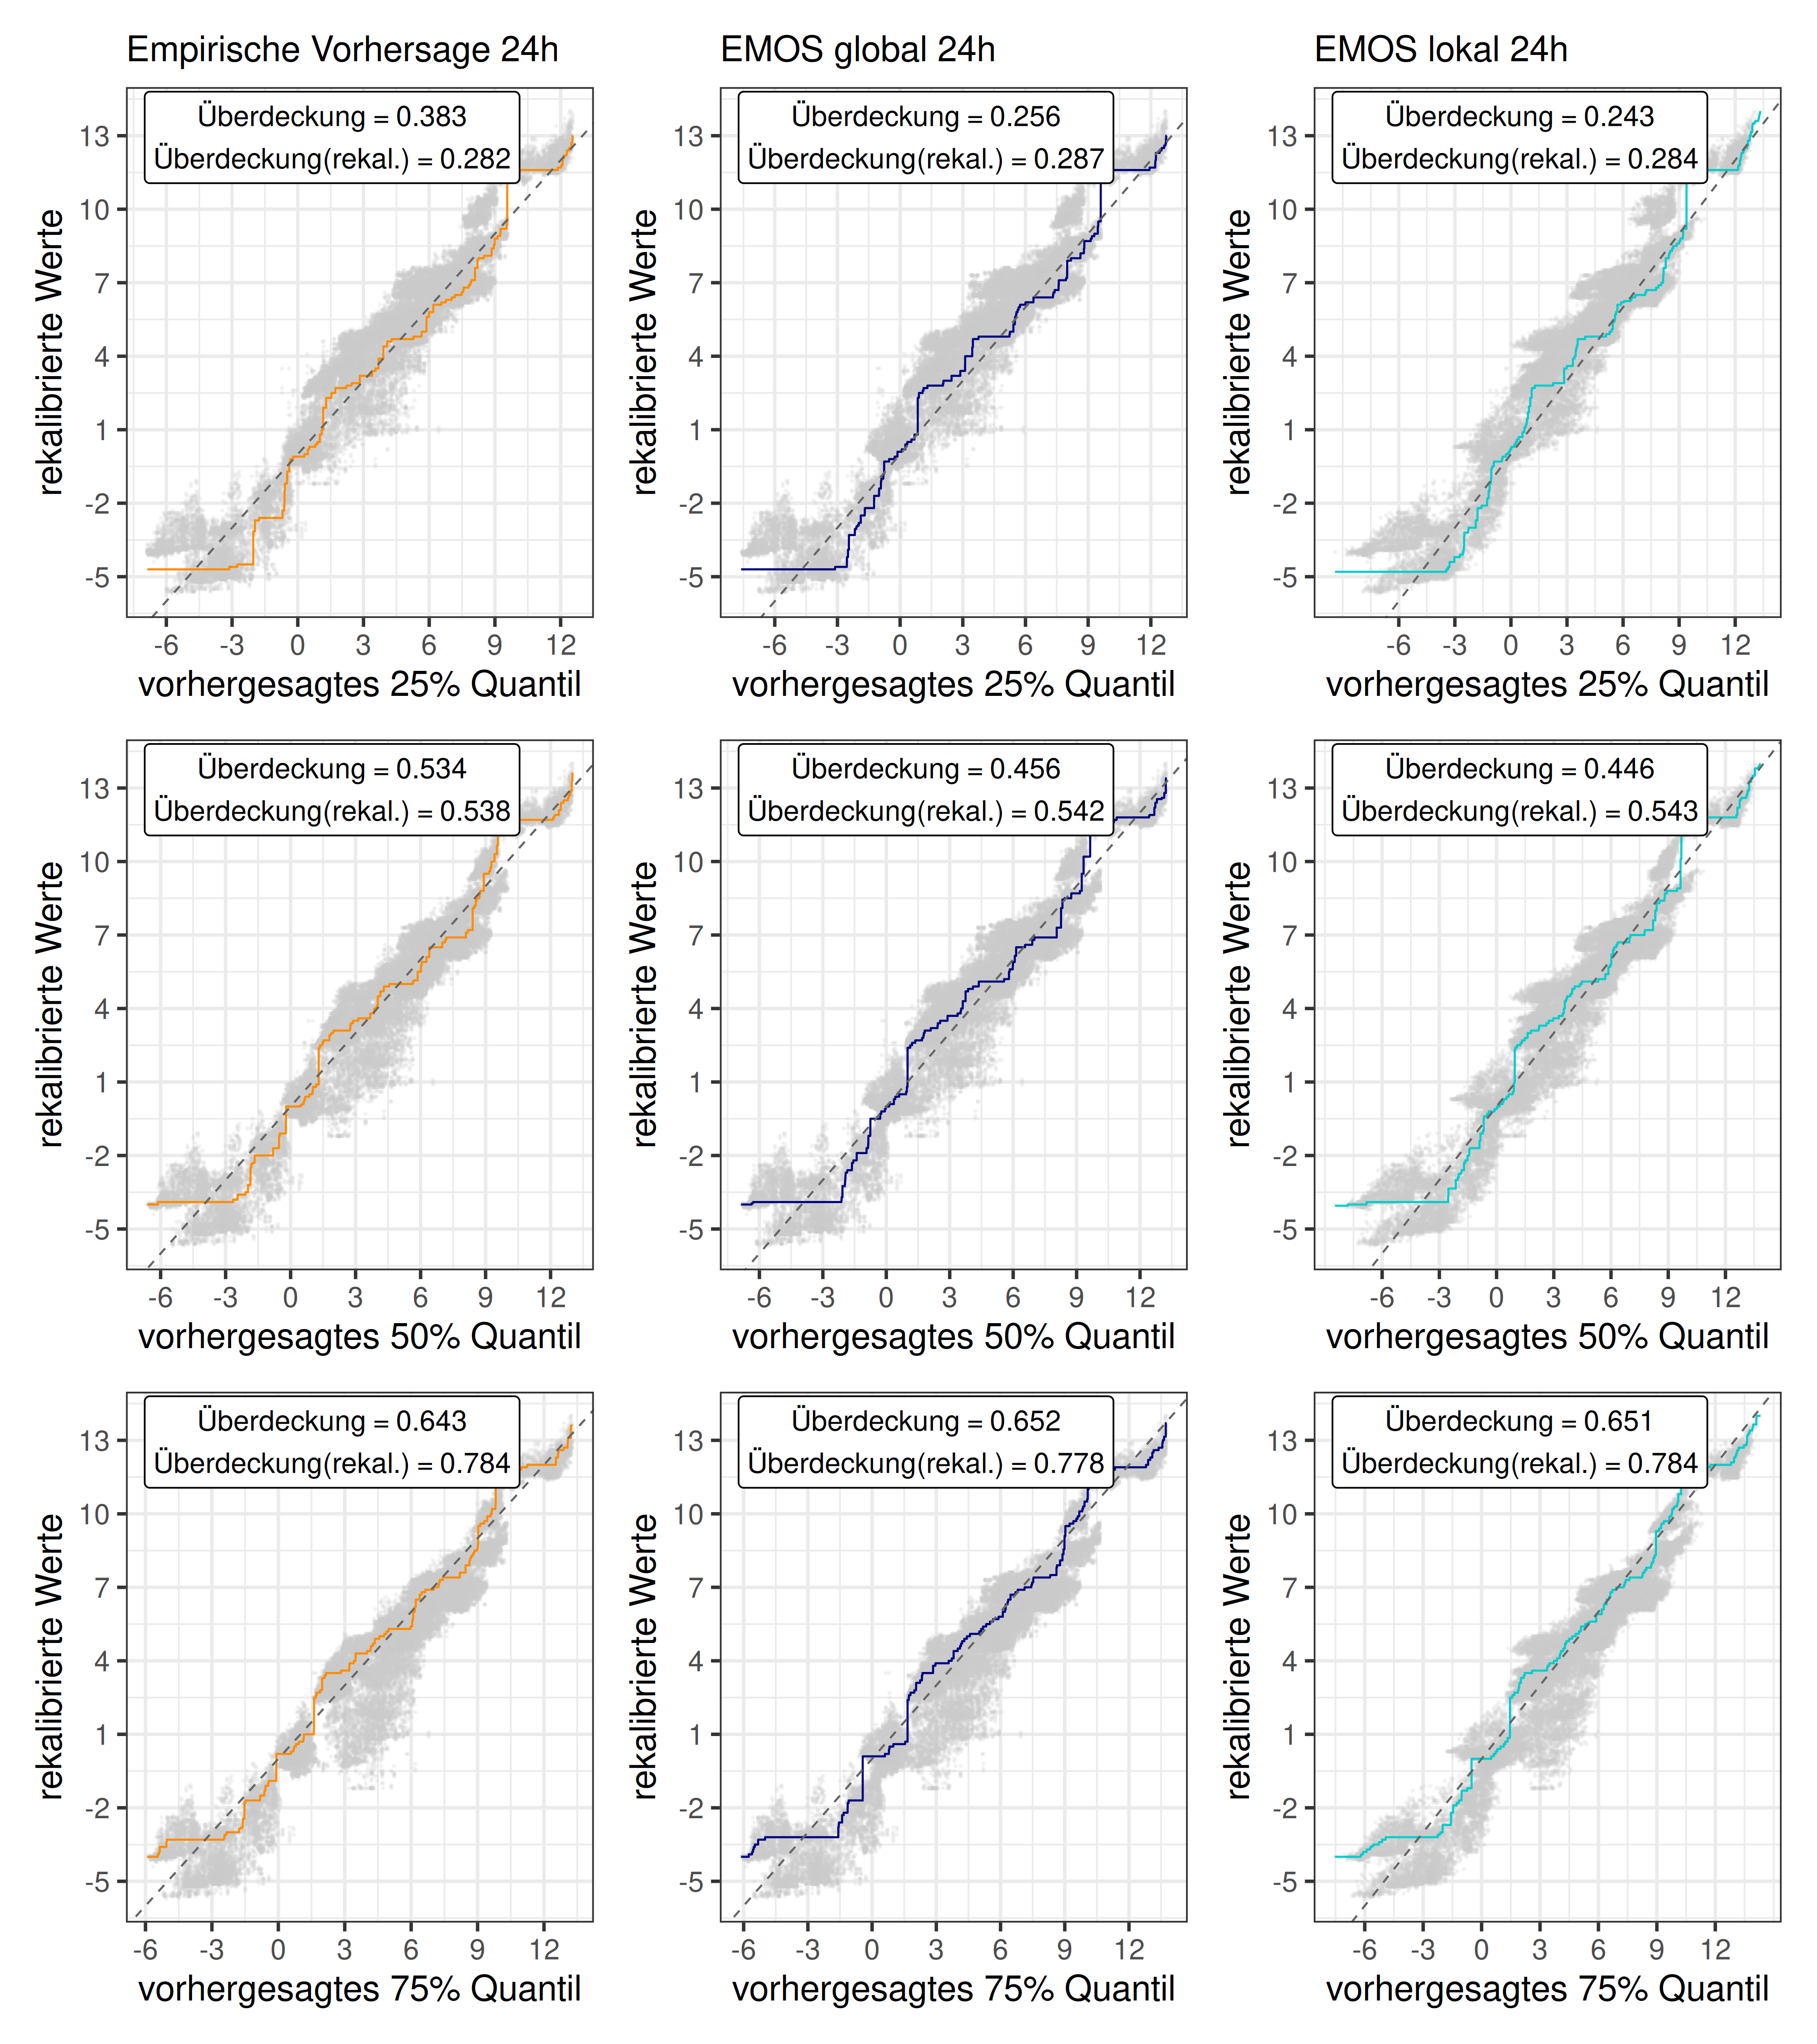
\includegraphics[width=\linewidth]{figs/quant_24_Rplot.png}
    \caption{Reliabilitätsdiagramme der Quantilkalibrierung für den Vorhersagehorizont $24\h$ für die Quantile $25\%$, $50\%$ und $75\%$. Die Plots sind zeilenweise nach Quantilniveau und spaltenweise nach Vorhersageverfahren angeordnet.}
    \label{fig:quant_plot}
\end{figure}

\begin{figure}[!h]
    \centering
    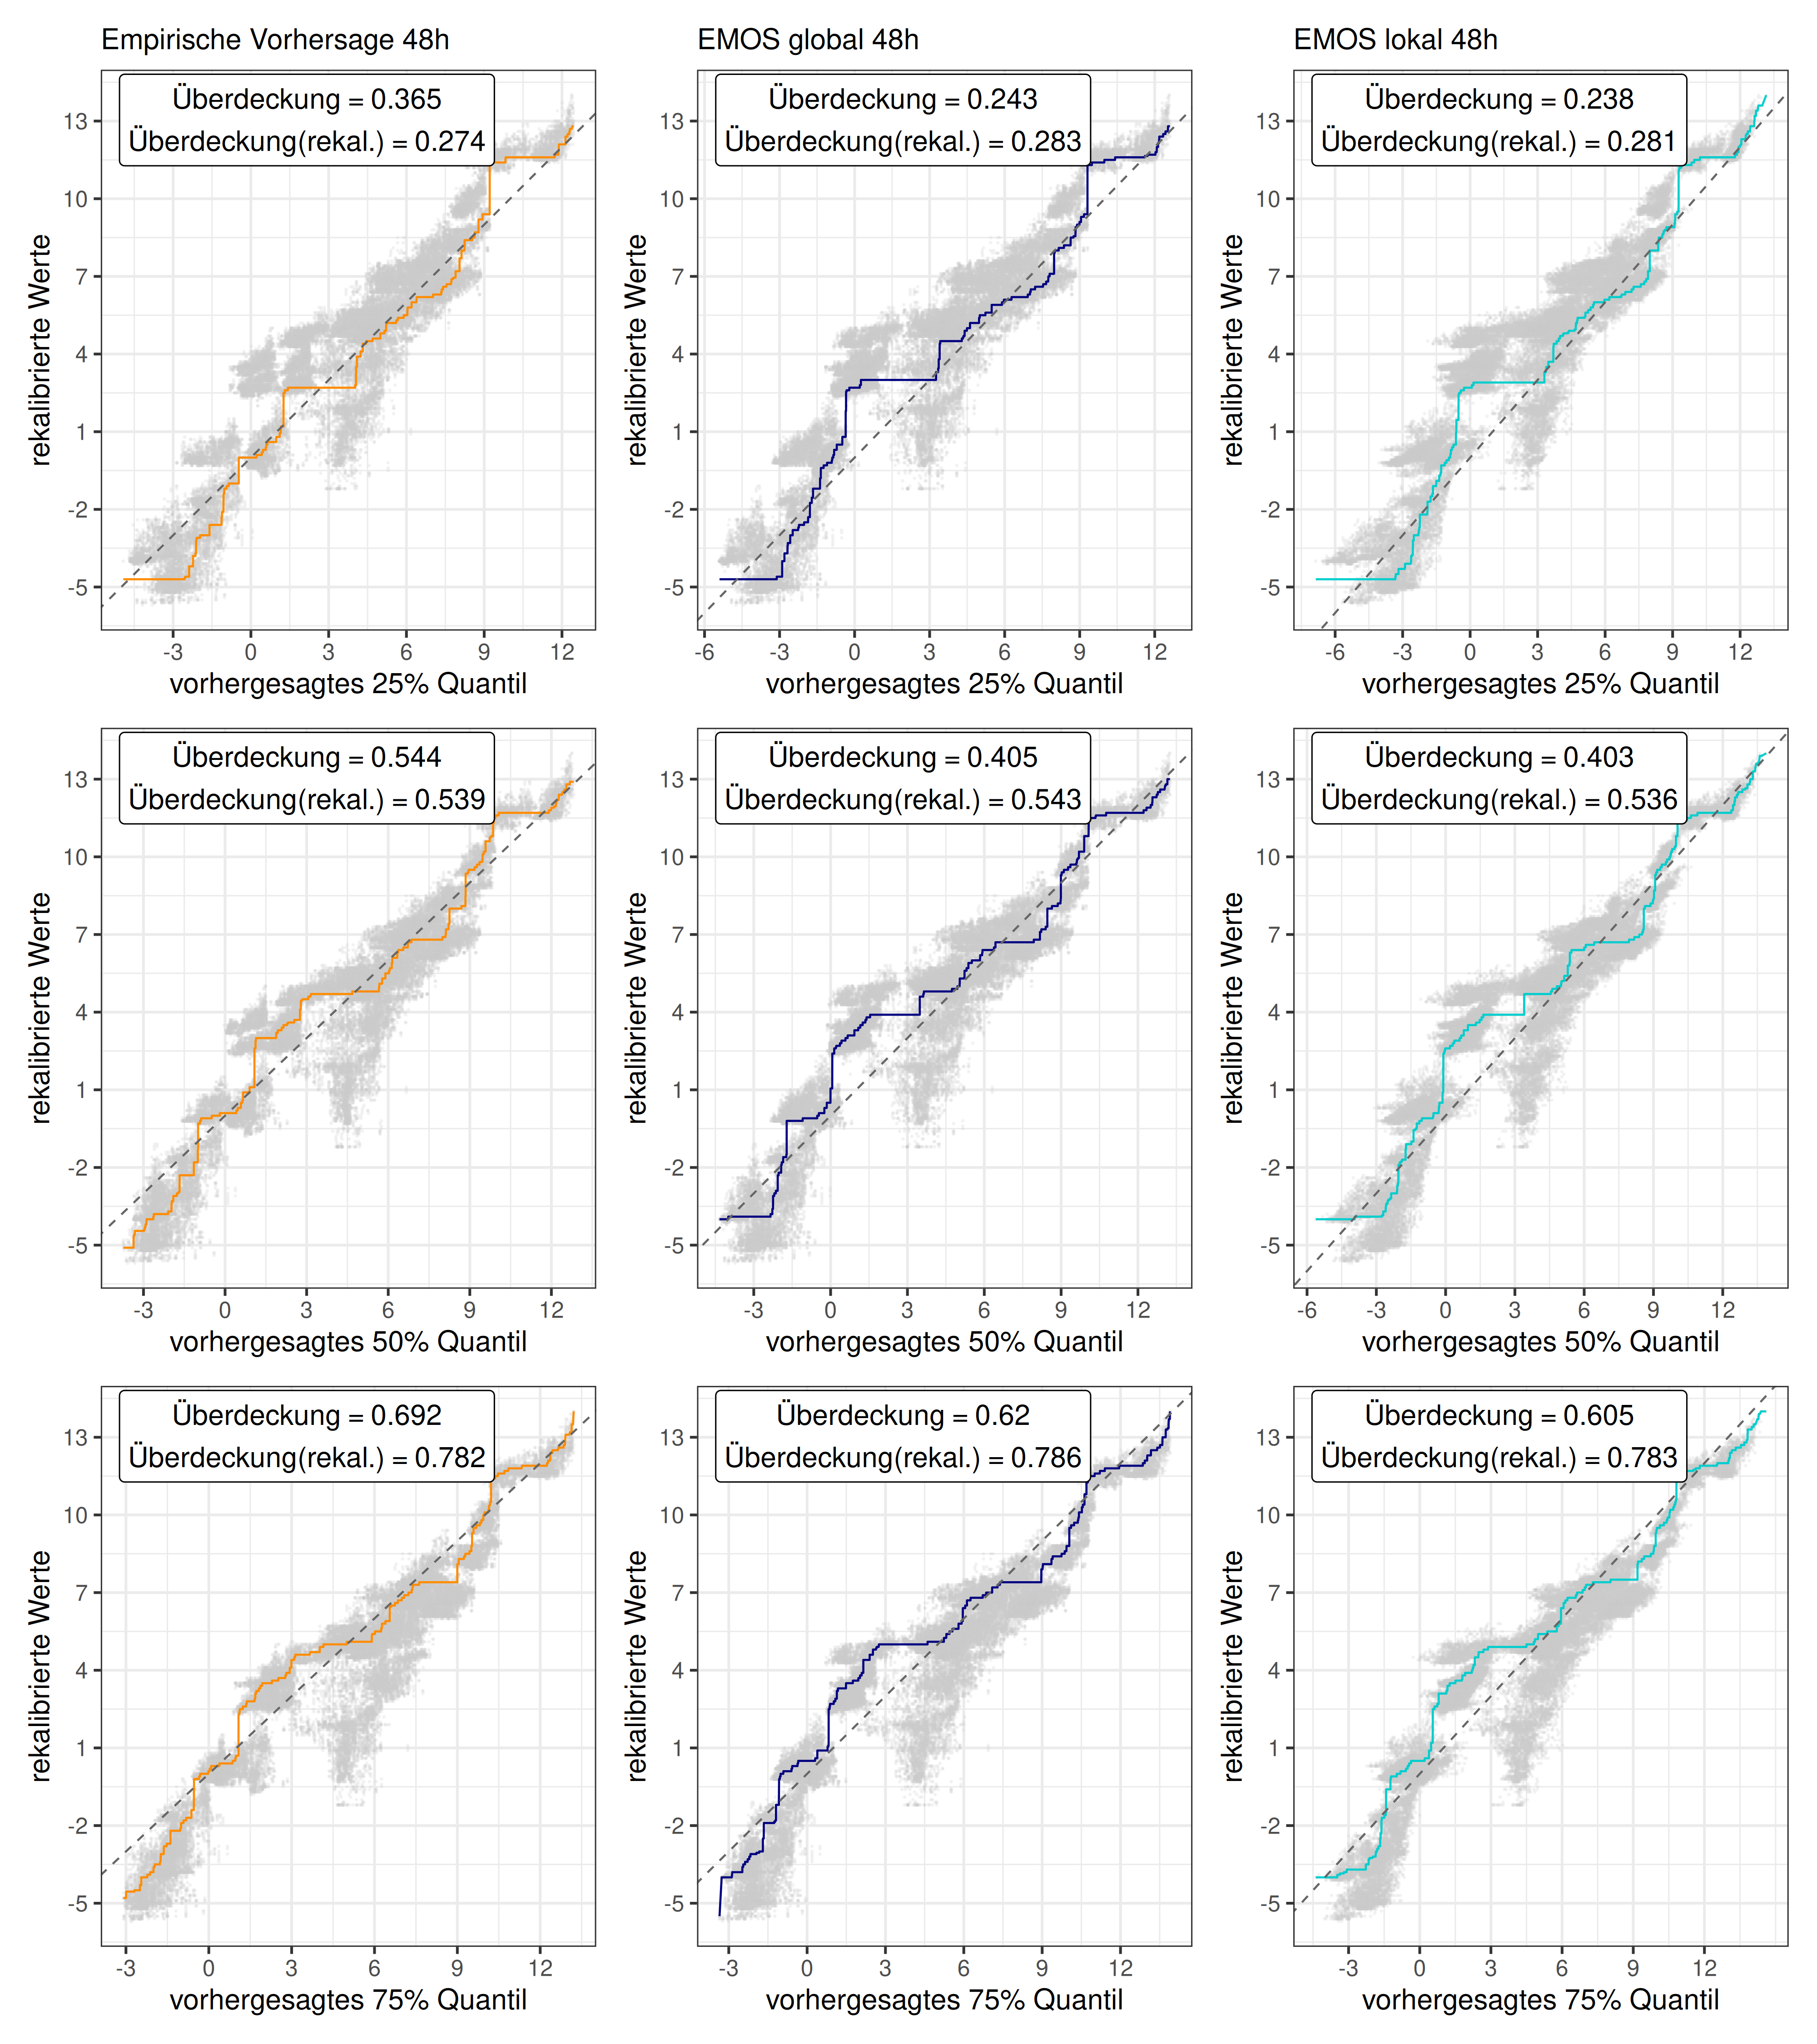
\includegraphics[width=\linewidth]{figs/quant_48_Rplot.png}
    \caption{Reliabilitätsdiagramme der Quantilkalibrierung für den Vorhersagehorizont $48\h$ für die Quantile $25\%$, $50\%$ und $75\%$. Die Plots sind zeilenweise nach Quantilniveau und spaltenweise nach Vorhersageverfahren angeordnet.}
    \label{fig:quant_48_plot}
\end{figure}

Für den Vorhersagehorizont $24\h$ ist über alle drei Vorhersagen hinweg eine ähnliche Fehlerstruktur erkennbar. Insgesamt verlaufen die Kalibrierungsfunktionen im zentralen Wertebereich relativ nahe an der Diagonalen. Abweichungen treten insbesondere in den unteren Randbereichen auf. Im Bereich kleiner vorhergesagter Quantile zeigen sich längere horizontale Segmente der Kalibrierungsfunktion. Dies deutet auf eine erhöhte Anzahl an Monotonieverletzungen hin, wodurch die Quantilkalibrierung im unteren Wertebereich nicht optimal ist. Vorhergesagte Quantile unterhalb von etwa $-5\C$ unterschätzen die beobachteten Quantile, während Quantilvorhersagen zwischen etwa $-4\C$ und $0\C$ sie überschätzen. Darüber hinaus zeigen die EMOS-Vorhersagen im mittleren Temperaturbereich zwischen etwa $1\C$ und $5\C$ eine leichte Unterschätzung der bedingten beobachteten Quantile.

Zum Vorhersagehorizont $48\h$ zeigt sich ebenfalls eine ähnliche Struktur über alle Quantile und Vorhersagen. Im Bereich kleiner vorhergesagter Quantile sind die horizontalen Abschnitte zwar weniger ausgeprägt als beim $24\h$ Horizont, dennoch liegen die rekalibrierten Werte überwiegend unterhalb der Diagonalen. Die vorhergesagten Quantile in diesem Wertebereich überschätzten somit die beobachteten Quantile. Auffällig ist erneut, dass die Kalibrierungskurven der EMOS-Vorhersagen im Temperaturbereich zwischen $0\C$ und $5\C$ oberhalb der Diagonalen liegen. Diese Abweichung ist im Vergleich zum $24\h$ Horizont deutlich stärker ausgeprägt. Das weist auf eine Unterschätzung der beobachteten Quantile in diesem Temperaturbereich hin.


%Marginale Kalibrierung:
%24 h: alle Vorhersagen ähnlich gut, empirische Vorhersage mit geringsten Abweichungen
%48 h: EMOS schlechter als empirische Vorhersage
%Probabilistische Kalibrierung:
%24 h: EMOS insgesamt besser als Rohensemble (weniger Unterdispersion), aber mit negativem Bias
%48 h: EMOS keine Verbesserung 
%Quantilkalibrierung:
%24 h: ähnliche Qualität, empirische Vorhersage eventuell leicht besser (wegen  Abweichungen im Bereich 1{-}5
%48 h: empirische Vorhersage besser aufgrund geringerer systematischer Abweichungen im Bereich 1{-}5


\FloatBarrier
\section{Scores} \label{sec:res_scores}

\subsection{CRPS und Quantilscore}


Tabelle \ref{tab:crps} fasst den mittleren CRPS der Vorhersagen über alle Zeitpunkte und Gitterzellen zusammen. Die Scores reichen von minimal $0.05\C$ bis maximal $5.53\C$. Für den $24\h$ Horizont unterscheiden sich die Vorhersagen mit einem Wert von etwa $0.6\C$ kaum, nur das die lokale Vorhersage einen geringeren maximalen Score aufweist. Für den $48\h$ Horizont liefert die empirische Vorhersage die besten Ergebnisse ($0.81\C$). Die EMOS Vorhersagen sind um etwa $0.1\C$ schlechter.

\begin{table}[!h]
\caption{CRPS der Vorhersagen.}
\centering
\newcolumntype{L}{>{\raggedright\arraybackslash}X}
\newcolumntype{R}{>{\raggedleft\arraybackslash}X}
\begin{tabularx}{0.9\textwidth}{L L R R R R}
\toprule
Horizont & Methode & CRPS & Min & Max & $q_{25}$--$q_{75}$\\
\midrule
\addlinespace[0.3em]
\multicolumn{6}{l}{24 h\,h}\\
& empirisch & 0.64 & 0.05 & 5.53 & 0.23--0.90\\
& global & 0.63 & 0.16 & 5.09 & 0.28--0.83\\
& lokal & 0.62 & 0.09 & 3.80 & 0.26--0.83\\
\addlinespace[0.3em]
\multicolumn{6}{l}{48 h\,h}\\
& empirisch & 0.81 & 0.05 & 5.61 & 0.30--1.13\\
& global & 0.90 & 0.16 & 5.05 & 0.37--1.30\\
& lokal & 0.91 & 0.09 & 4.90 & 0.37--1.32\\
\bottomrule
\end{tabularx}
\label{tab:crps}
\end{table}


Als Nächstes untersuchen wir, wie sich die Güte der Vorhersagen über verschiedene Quantilniveaus hinweg verhält. Dazu zeigt Abbildung \ref{fig:qs_plot} den verdoppelten mittleren Quantilscore in Abhängigkeit vom Quantilniveau der Vorhersagen, sodass die Fläche unter der Kurve dem mittleren CRPS der jeweiligen Vorhersage entspricht (vgl. Abschnitt \ref{seq:crps_qs}). Dadurch lässt sich identifizieren, welche Quantilbereiche Unterschiede im CRPS verursachen. Es zeigt sich ein typischer umgekehrter U-förmige Verlauf des Quantilscores: Die Randquantile weisen geringere Scores auf, während die größten Beiträge zum CRPS aus dem mittleren Quantilbereich stammen.

Für den Vorhersagehorizont $24\h$ unterscheiden sich die Verfahren insgesamt nur geringfügig: Die größten Abweichungen treten im unteren und mittleren Quantilbereich auf. Während die EMOS-Vorhersagen im unteren Bereich geringfügig bessere Quantilscores aufweisen, erzielt die empirische Vorhersage im mittleren Bereich leicht bessere Werte. Für den Vorhersagehorizont von $48\h$ sind die EMOS-Vorhersagen bis etwa zum $25\%$-Quantilniveau zwar ebenfalls geringfügig überlegen, weisen jedoch für alle höheren Quantilniveaus deutlich schlechtere Scores auf. Die Defizite der EMOS-Vorhersagen diesen Horizonts liegen somit insbesondere in den höheren Quantilbereichen.

%Dies erklärt insbesondere die erhöhten Quantilscores im Bereich hoher Quantile, da extreme Beobachtungen durch die Vorhersagen nicht ausreichend abgebildet werden.
 
\begin{figure}[!h]
    \centering
    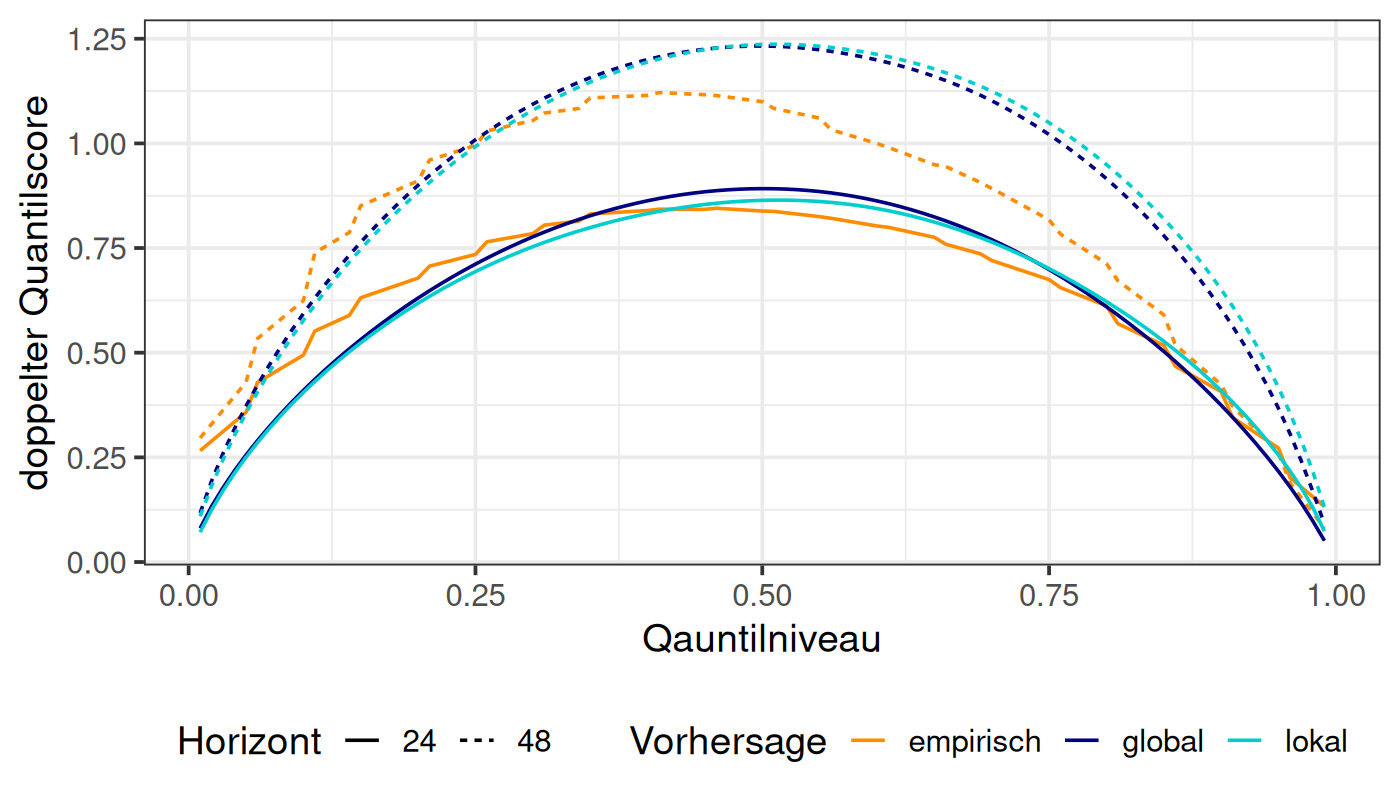
\includegraphics[width=.75\linewidth]{figs/qs_error_curve_Rplot.png}
    \caption{Doppelter Quantilscore für verschiedene Qauntilniveaus der Vorhersagen.}
    \label{fig:qs_plot}
\end{figure}




\subsection{Score Zerlegung}
Zur Analyse von Quellen der Vorhersagequalität wurde der mittlere CRPS, wie in Kapitel \ref{chap:score_decomp} erläutert, in die Komponenten Unsicherheit (UNC), Diskriminationsfähigkeit (DSC) und Misskalibrierung (MCB) zerlegt. Zusätzlich wurde der mittlere Quantilscore für die Niveaus $25\%$, $50\%$ und $75\%$ sowie die extremen Quantile $5\%$ und $95\%$ ebenfalls zerlegt, um die Vorhersagequalität für verschiedene Bereiche der Vorhersageverteilung zu analysieren. Der Quantilscore ist wieder verdoppelt, um ihn besser mit dem CRPS vergleichen zu können (vgl. \eqref{eq:crps_qs}).

%\todo{hier vielleicht mit shape und color statt textstring arbeiten}
\begin{figure}[!htbp]
    \centering
    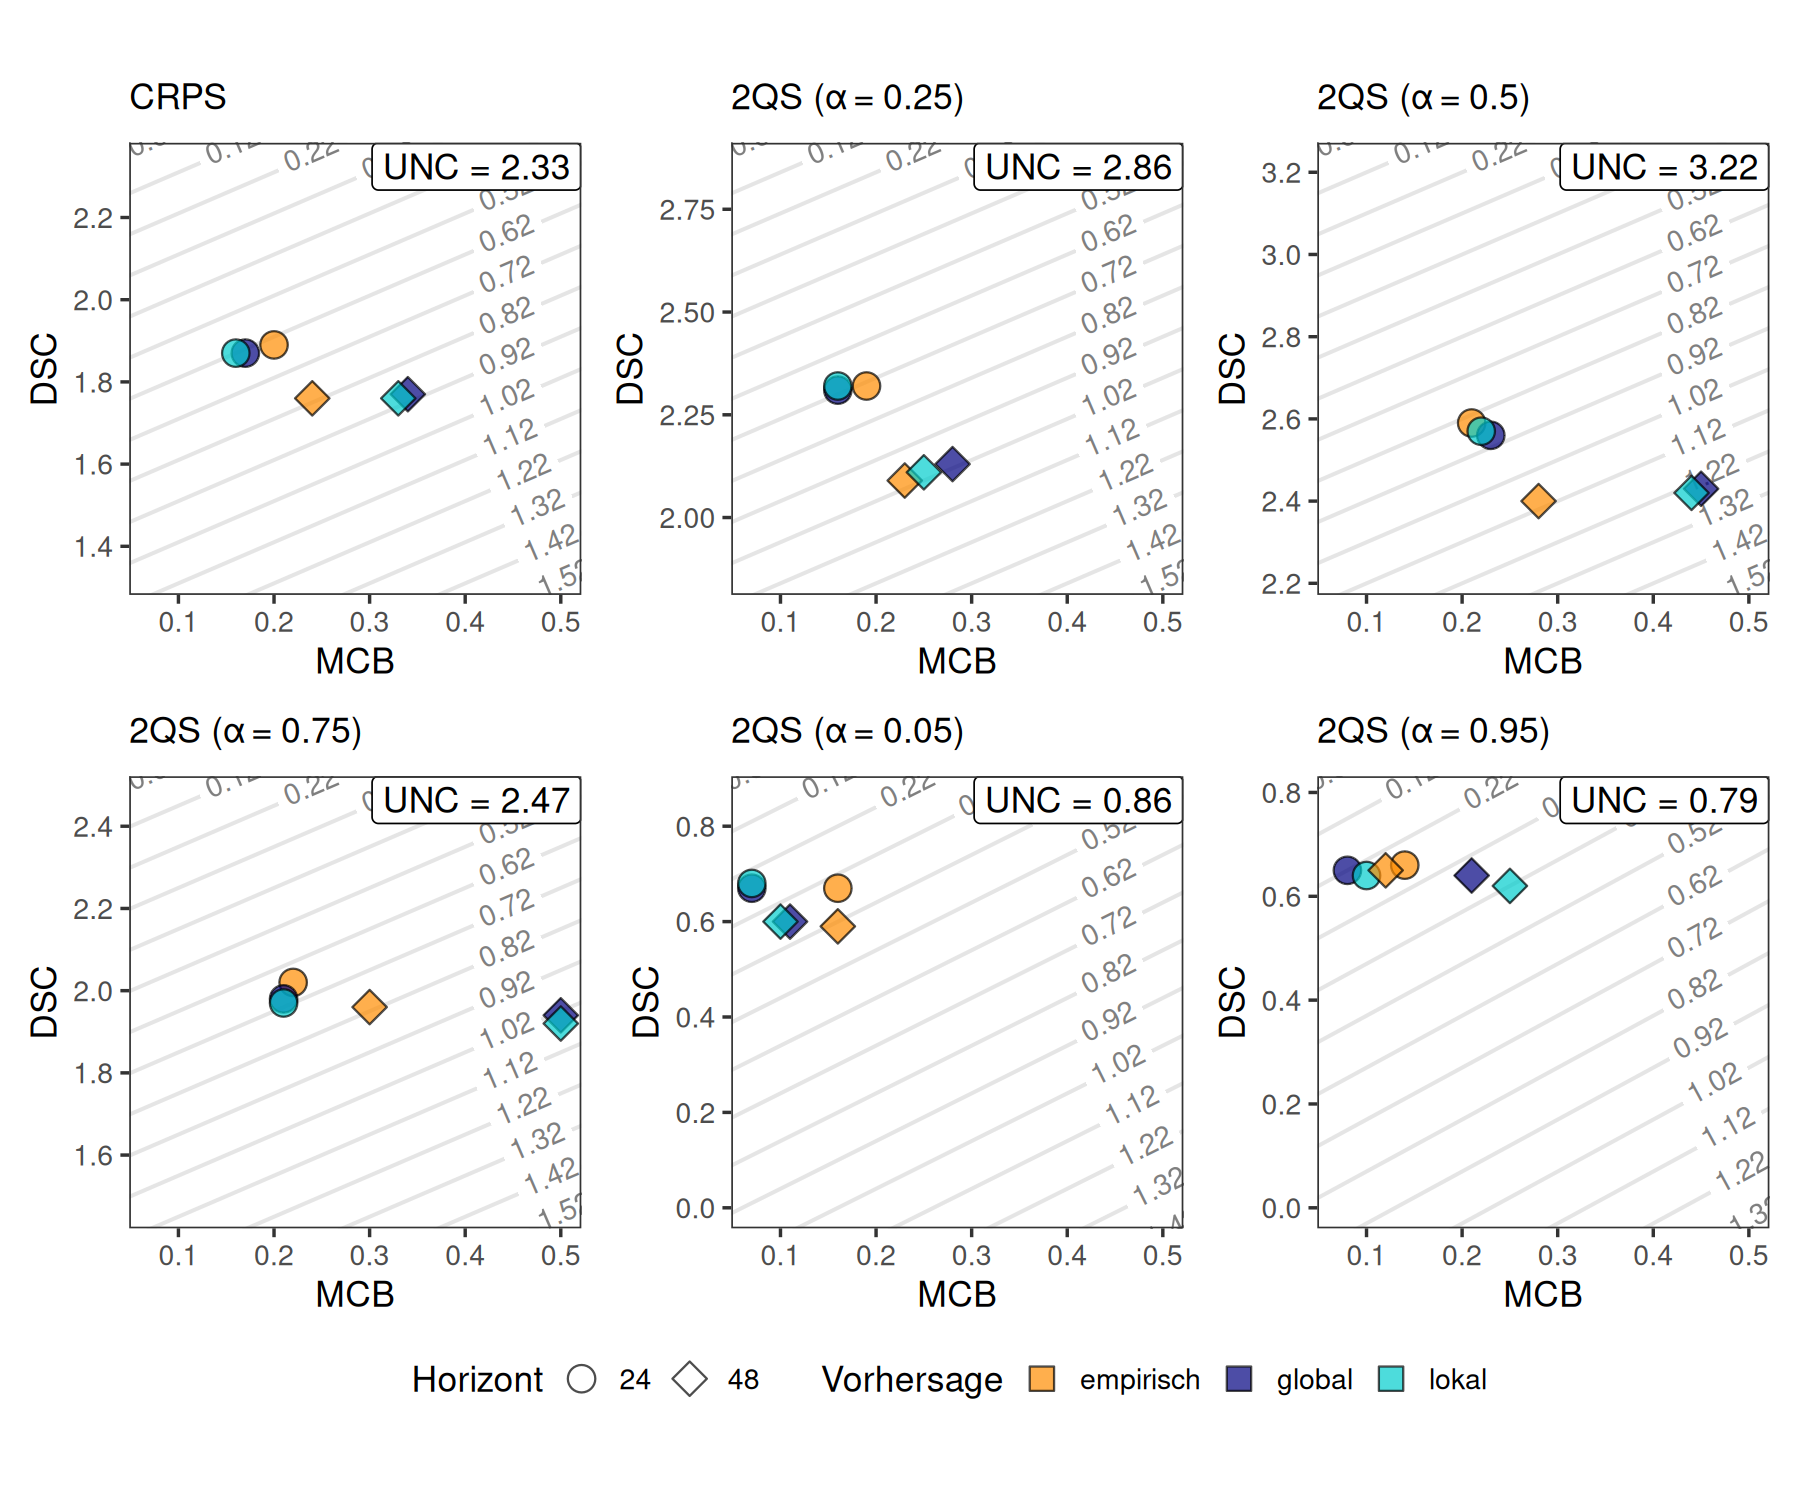
\includegraphics[width=1\linewidth]{figs/decomp_Rplot.png}
    \caption{Zerlegungsdiagramme der Scores.}
    \label{fig:decomp_plot}
\end{figure}

%Für $48\h$ verschlechtern sich sowohl Kalibrierung als auch Diskriminierung.
Abbildung \ref{fig:decomp_plot} zeigt die Zerlegungsdiagramme für die verschiedenen Scores. Die $24\h$ Vorhersagen zeigen für fast alle Scores eine bessere Kalibrierung und Diskriminierung als die $48\h$ Vorhersagen vor allem hinsichtlich Kalibrierung. Zudem bestehen zwischen der globalen und der lokalen Vorhersage wieder geringe Unterschiede.

Der CRPS zeigt für $24\h$ nur geringe Unterschiede zwischen den Vorhersagen, wobei die EMOS-Vorhersagen minimal besser kalibriert, jedoch leicht schlechter diskriminierend sind. Für $48\h$ weisen die EMOS-Vorhersagen eine ähnliche Diskriminations\-fähigkeit wie die empirischen Vorhersage auf, jedoch sind sie schlechter kalibriert, wodurch der Gesamtscore schlechter wird. Die Quantilscores zeigen ein ähnliches Muster wie der CRPS, jedoch mit etwas größeren Scoreunterschieden. Beim $25\%$-Quantil sind die EMOS-Vorhersagen für den $48\h$ Horizont ähnlich der empirischen Vorhersage kalibriert, während sie beim $50\%$- und $75\%$-Quantil eine auffallend schlechtere Kalibrierung aufweisen. Die extremen Quantile ($5\%$ und $95\%$) zeigen die niedrigsten Scores, weisen jedoch auch die geringste Unsicherheitskomponente auf. Beim $5\%$-Quantil sind alle EMOS-Vorhersagen leicht besser kalibriert als die empirischen Vorhersagen. Beim $95\%$-Quantil entspricht das Verhalten weitgehend dem des $75\%$-Quantils, jedoch sind die Unterschiede in der Kalibrierung nicht so stark ausgeprägt. Die genauen Zahlen der Zerlegung mit dem Skill Score sind in Appendix \ref{seq:decomp-table} dargestellt.


\subsection{Räumliche und zeitliche Dynamiken im CRPS} \label{sec:res_spat_time}
Die Analyse der räumlichen und zeitlichen Dynamiken der Vorhersagen im CRPS ermöglicht eine Bewertung, wie sich die Qualität der Temperaturvorhersagen über verschiedene Regionen und Vorhersagezeiträume hinweg verändert.

Abbildung \ref{fig:crps_day_plot} zeigt den mittleren CRPS über die Tage des Evaluationszeitraums getrennt nach Vorhersage. Über die verschiedenen Tage sind die Fehlerwerte ungleichmäßig verteilt, wobei sowohl Phasen mit vergleichsweise niedrigen als auch mit erhöhten CRPS-Werten auftreten. Die Scores reichen von $0.2\C$ bis über $2.5\C$. Wieder sind für den $48\h$ Horizont die Fehler deutlich größer. Auch zeigen die EMOS-Vorhersagen jeweils ein nahezu identisches Profil.

\begin{figure}[h]
    \centering
    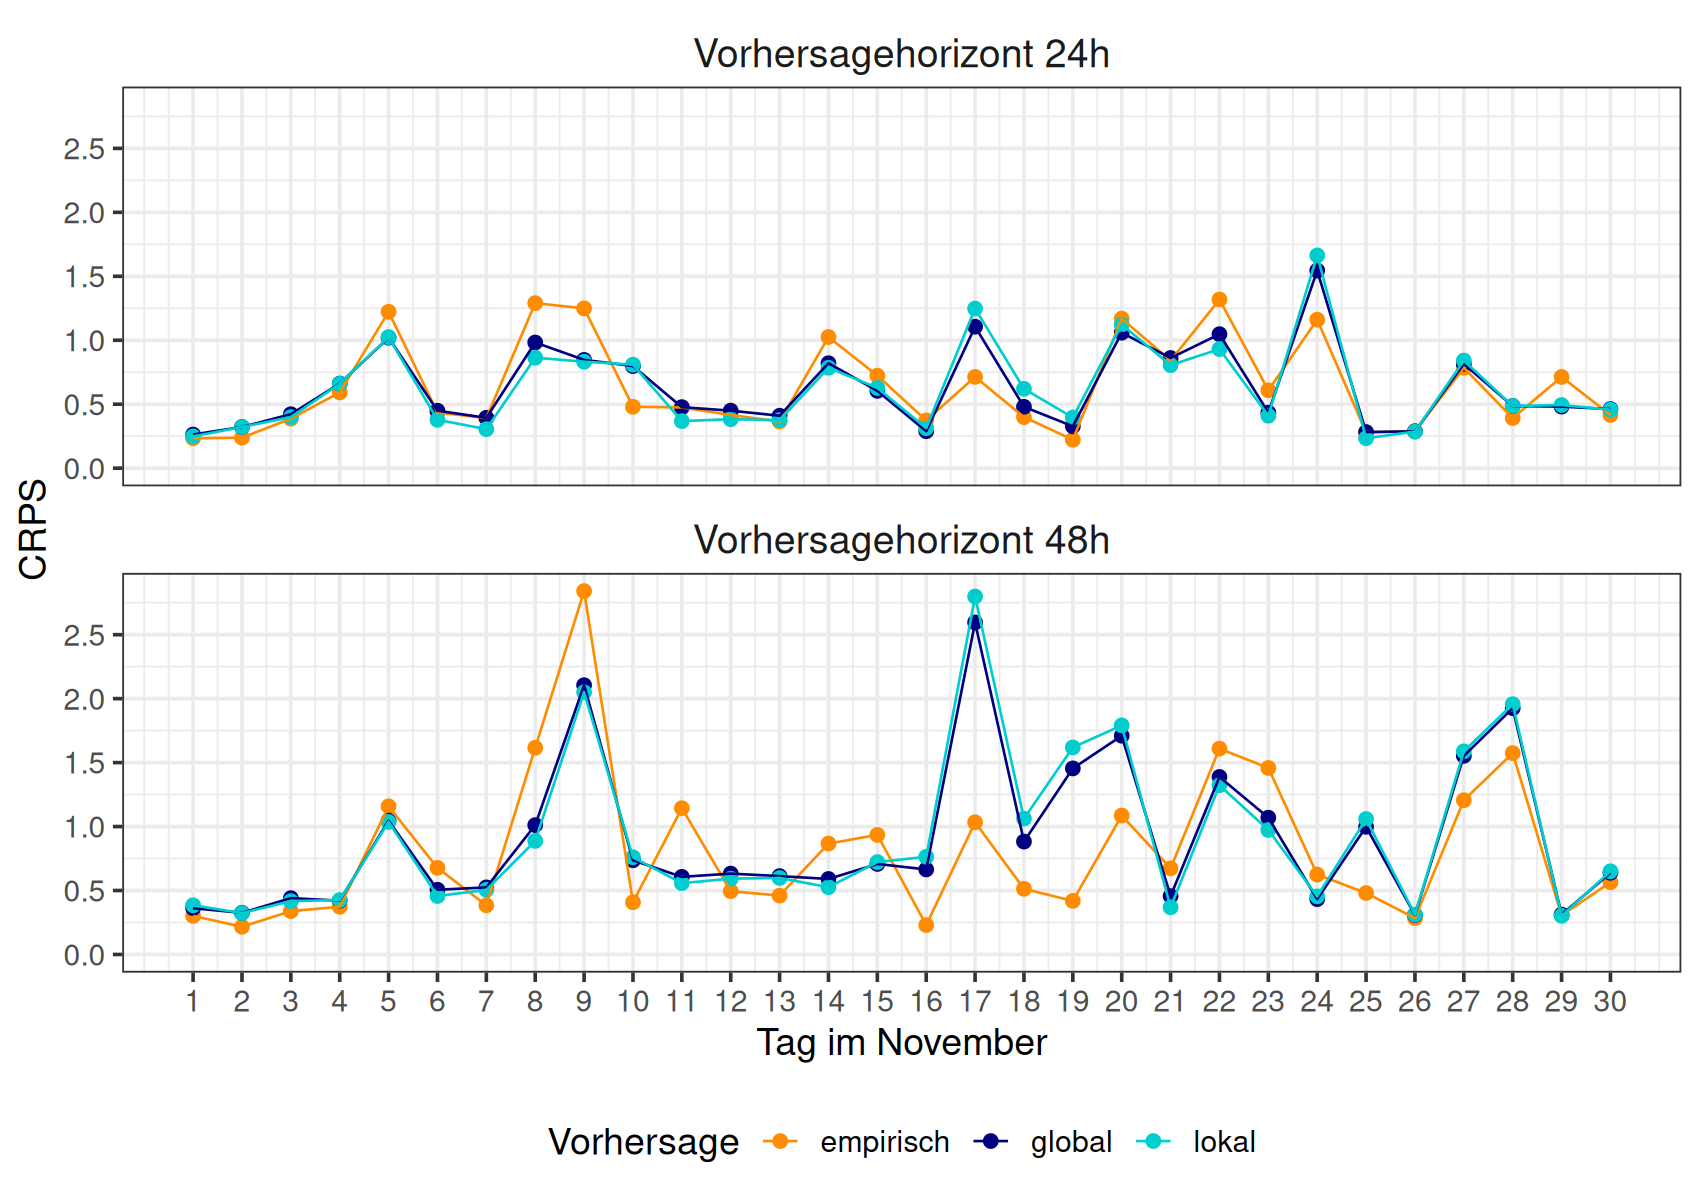
\includegraphics[width=0.9\linewidth]{figs/crps_time.png}
    \caption{Zeitlicher Verlauf des mittleren CRPS über den Evaluationszeitraum.}
    \label{fig:crps_day_plot}
\end{figure}

Für den $24\h$ Horizont liegen alle Vorhersagen recht nah beieinander, wohingegen sich beim $48\h$ die empirische und die EMOS-Vorhersagen stärker voneinander unterscheiden. Besonders fällt auf, dass über beide Vorhersagehorizonte die EMOS-Vorhersagen am 17.11. Scores besitzen, die schlechter sind als die der korrespondierenden empirischen Vorhersagen. Dieses Muster lässt sich durch den negativen Bias der EMOS-Vorhersagen erklären (vgl. Abschnitt \ref{sec:res_pit_cal}). So fällt im Vergleich mit Abbildung \ref{fig:icon_time} auf, dass die EMOS-Vorhersagen tendenziell einen höheren CRPS aufweisen, wenn viele Ensemblemitglieder unter der HOSTRADA-Temperatur liegen, also zu niedrig sind. Liegen viele Ensemblemitglieder unter der HOSTRADA-Temperatur, führt der negative Bias der EMOS-Vorhersage zu einer stärkeren Unterschätzung der Temperatur und somit zu einer größeren Abweichung von der beobachteten Temperatur, was sich in einem höheren CRPS widerspiegelt. Die empirische Vorhersage weist dagegen bei beiden Vorhersagehorizonten am 9.11. und 22.11. die höchsten Scores auf. Der Vergleich mit Abbildung \ref{fig:icon_time} zeigt, dass die Ensemblemitglieder an diesen Tagen die HOSTRADA-Temperatur tendenziell überschätzen.

Um räumliche Variationen in der Vorhersagegüte zu erfassen, ist in Abbildung \ref{fig:crps_cells} der mittlere CRPS pro Gitterzelle dargestellt. Für den Horizont $24\h$ weisen alle Vorhersagen überwiegend niedrige CRPS-Werte zwischen etwa $0.4\C$ und $0.8\C$ auf, was auf eine gute Übereinstimmung zwischen Vorhersage und Beobachtung hindeutet. Bei $48\h$ steigen die CRPS-Werte in allen Vorhersagen deutlich an.

Über alle Vorhersagen hinweg lassen sich folgende räumliche Muster erkennen. Im östlichen bzw. südöstlichen Berliner Randgebiet treten erhöhte CRPS-Werte auf, während im westlichen und zentralen Bereich geringere Fehler beobachtet werden. Insbesondere fallen bei den empirischen Vorhersagen Fehlerhotspots auf. Diese korrespondieren mit Gewässern in Berlin, dem Teglersee (links oben), der Havel (links unten) und dem Großen Müggelsee (rechts unten) (siehe Abbildung \ref{fig:berlin_spat}). Hier unterscheidet sich die lokale Vorhersage von den anderen Verfahren. Sie glättet die zuvor beobachteten Hotspots räumlich.

Diese räumliche Systematik deutet nicht notwendig auf Defizite in der Vorhersagequalität hin, sondern könnte auf Unterschiede in der Modellierung der zugrunde liegenden Datensätze zurückzuführen sein. HOSTRADA stellt einen rasterbasierten Beobachtungsdatensatz dar, dessen Temperaturfelder überwiegend durch statistische Interpolation von Stationsmessungen erzeugt werden \parencite{krahenmann_high-resolution_2018}. Die Unterscheidung zwischen Wasser und Land erfolgt dabei über die Rauhigkeit der Fläche, wobei Wasserflächen eine sehr geringe Rauhigkeit zugewiesen bekommen. Dies beeinflusst die Windgeschwindigkeit und dadurch auch die Temperatur. Demgegenüber basiert ICON-D2-ESP auf einem numerischen Wettermodell, in dem die Eigenschaften der Oberflächen explizit berücksichtigt werden \parencite{reinert2025icon_dwd}. Aufgrund der nativen räumlichen Auflösung von 2 km können Gewässerränder jedoch nur grob abgebildet werden, sodass einzelne Gitterzellen sowohl Land- als auch Wassereigenschaften enthalten können. Unterschiede oder Unsicherheiten bei der Darstellung dieser Oberflächeneigenschaften können sich ebenfalls auf die simulierten Temperaturen auswirken. Diese Aspekte wurden mir auf Anfrage von Arne Spitzer vom Deutscher Wetterdienst (DWD), per E-Mail erläutert (persönliche Kommunikation, 2026).

Vor diesem Hintergrund ist es plausibel, dass Gewässer wie der Große Müggelsee im ICON-D2-ESP einen stärkeren Einfluss auf das Temperaturfeld ausüben als im HOSTRADA, der diese möglicherweise nur eingeschränkt abbildet. Ein Indiz hierfür ist, dass in Abbildung \ref{fig:nov_temp_spat} die Gewässer in den Temperaturbeobachtungen nicht sichtbar werden. Die an den Gewässern auftretenden erhöhten CRPS-Werte der Vorhersagen könnten somit zumindest teilweise auf Unterschiede in der Darstellung der Gewässer zwischen den beiden Datensätzen zurückzuführen sein.

\begin{figure}[h]
    \centering
    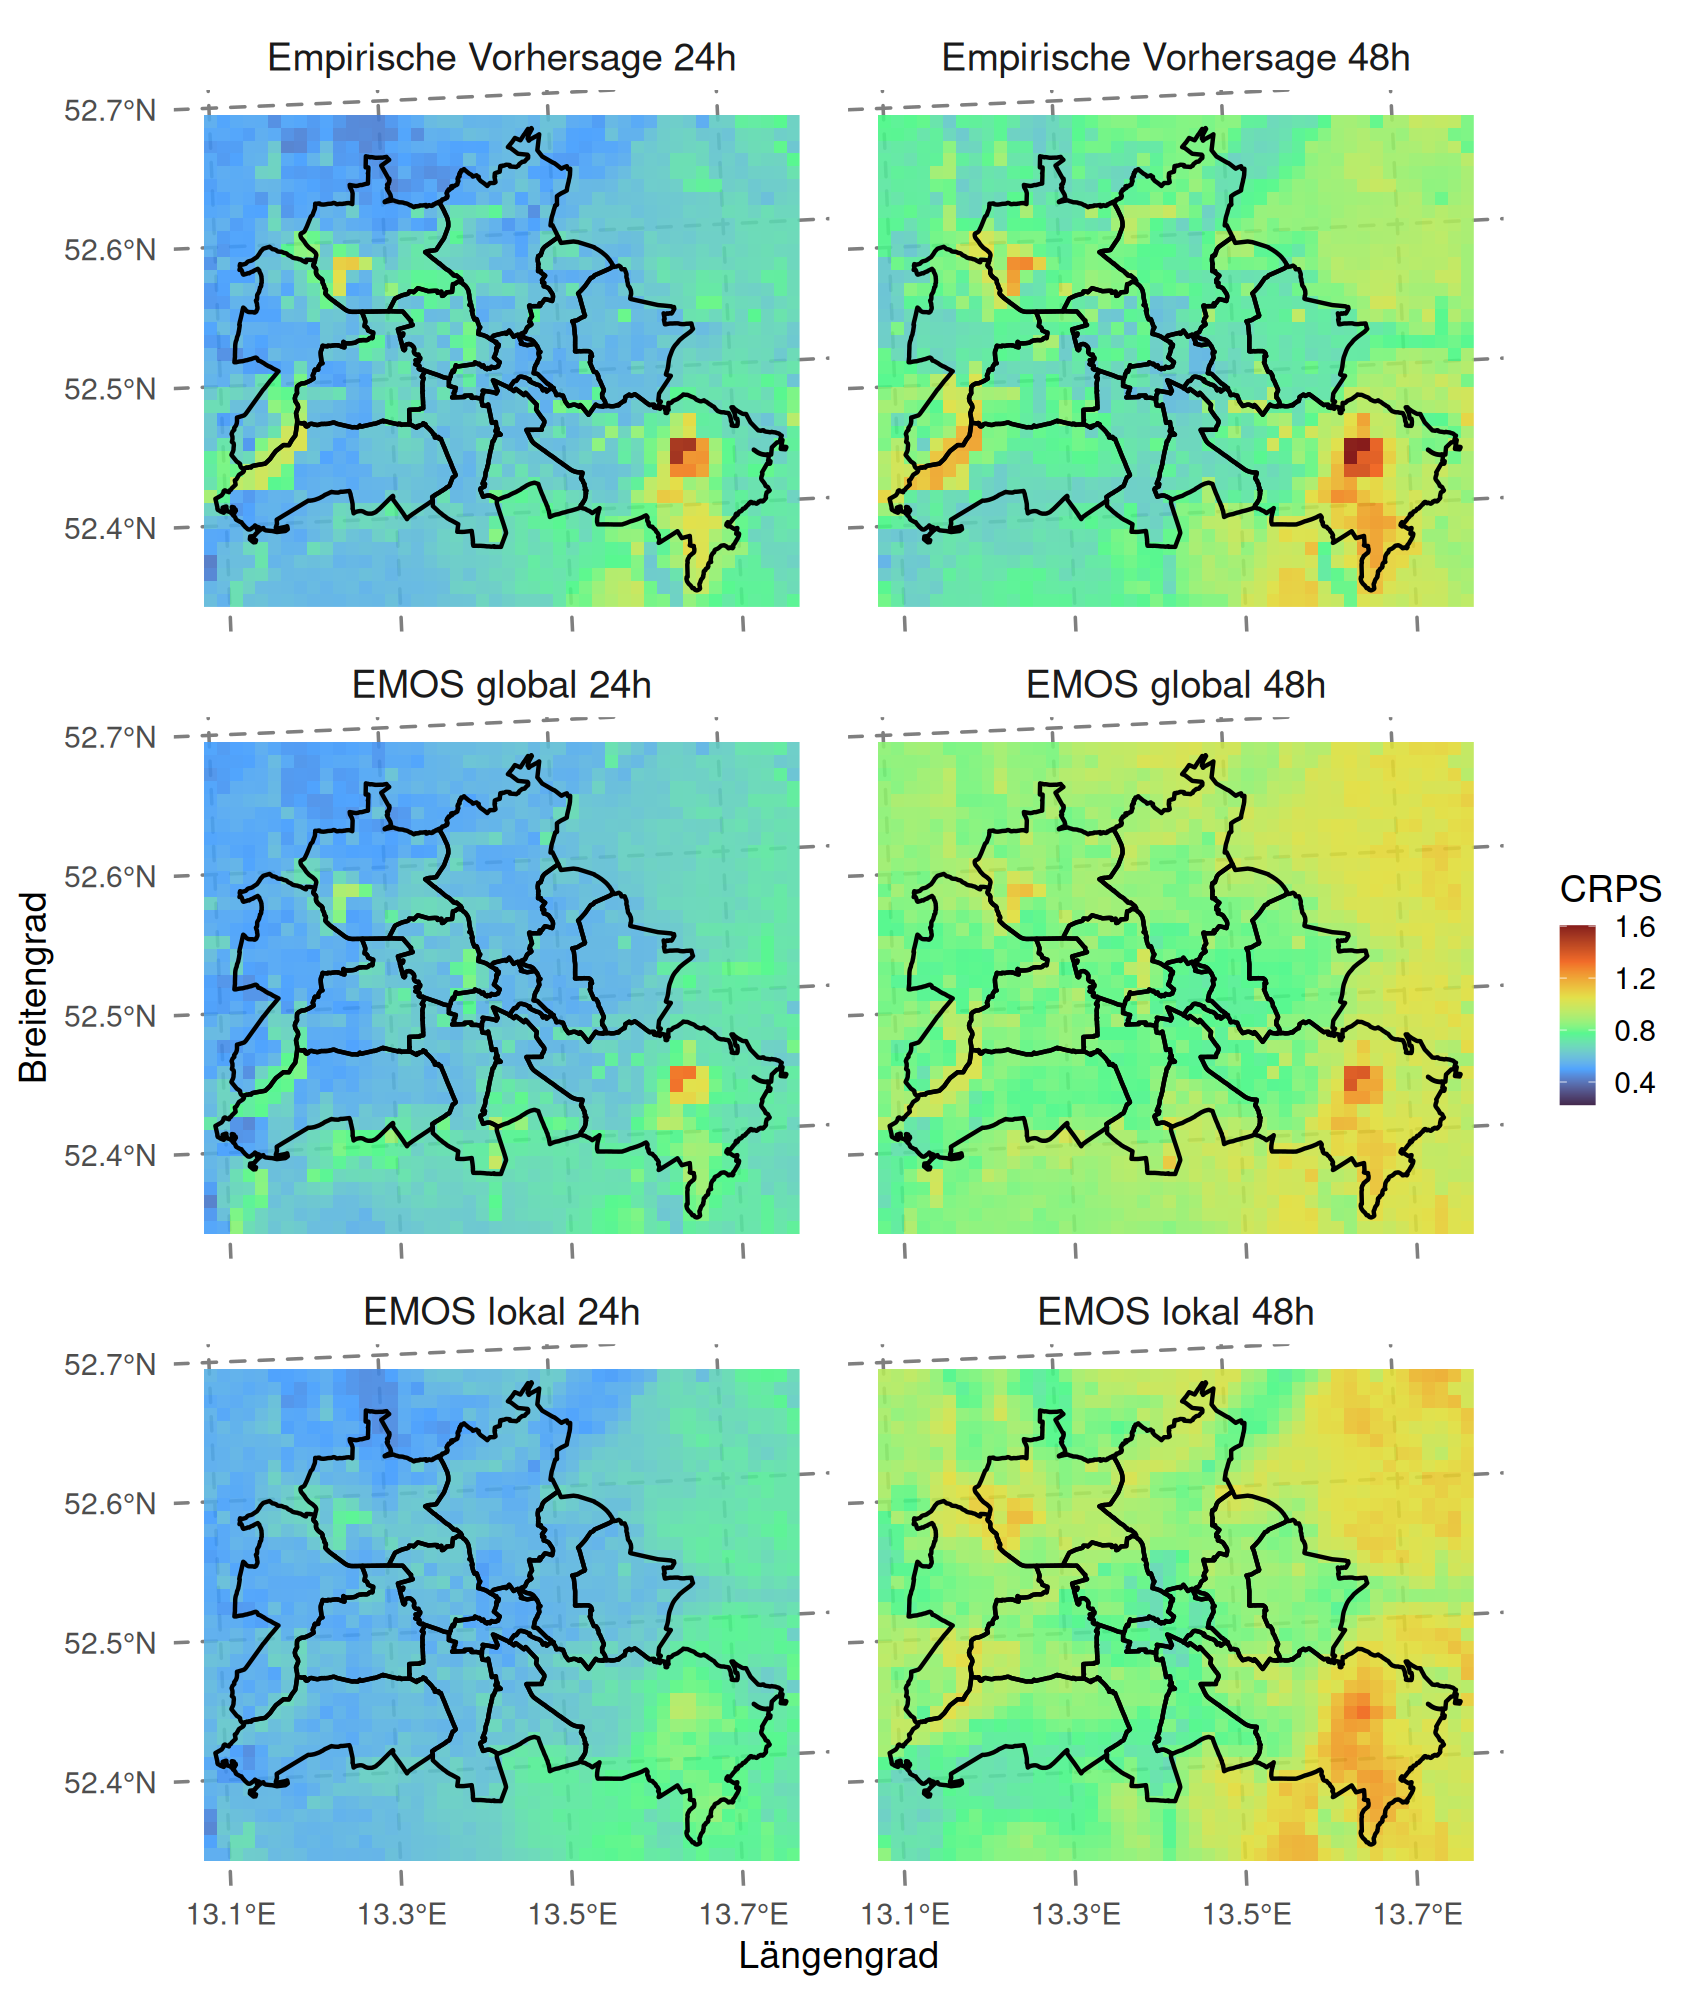
\includegraphics[width=0.89\linewidth]{figs/crps_spat.png}
    \caption{Mittlerer CRPS der Gitterzellen über den Evaluationszeitraum.}
    \label{fig:crps_cells}
\end{figure}


\FloatBarrier
\section{Zusammenfassung} \label{sec:res_sum}
Zusammenfassend zeigen die verschiedenen Kalibrierungsbegriffe ein differenziertes Bild. Die beiden EMOS-Vorhersagen unterscheiden sich dabei nur geringfügig und können daher weitgehend gemeinsam betrachtet werden. Hinsichtlich der marginalen Kalibrierung weisen für den $24\h$ Horizont alle betrachteten Vorhersagen eine vergleichbare Qualität auf, wobei die empirische Vorhersage die geringsten Abweichungen von der Idealgeraden in Abbildung \ref{fig:marg_plot} zeigt. Für den $48\h$ Horizont weisen die EMOS-Vorhersagen hingegen größere Abweichungen auf als die empirische Vorhersage.

Bei der probabilistischen Kalibrierung zeigt sich für den $24\h$ Horizont ein Vorteil der EMOS-Vorhersagen gegenüber der empirischen Vorhersage, weil die Unterdispersion der empirischen Vorhersage reduziert wird. Gleichzeitig tritt jedoch ein negativer Bias auf. Für den $48\h$ Horizont führt die EMOS-Vorhersage hingegen zu keiner Verbesserung der probabilistischen Kalibrierung, weil die Reduktion der Unterdispersion durch den stärkeren negativen Bias ausgeglichen wird.

Auch hinsichtlich der Quantilkalibrierung zeigt sich kein einheitlicher Vorteil der EMOS-Vorhersagen. Für den $24\h$ Horizont ist die Kalibrierung der betrachteten Vorhersagen insgesamt ähnlich. Für den $48\h$ Horizont weist die empirische Vorhersage hingegen eine bessere Quantilkalibrierung auf, weil bei den EMOS-Vorhersagen im Wertebereich von etwa $1\C$ bis $5\C$ Abweichungen von der Idealgraden auftreten. Insgesamt sind die betrachteten Vorhersagen als ausreichend kalibriert einzustufen, weisen jedoch weiterhin Abweichungen auf, insbesondere für den längeren Vorhersagehorizont von $48\h$.

Die Scoreanalysen bestätigen die bessere Vorhersagegüte des $24\h$ Horizonts gegenüber dem $48\h$ Horizont. Für den $24\h$ Horizont unterscheiden sich die Vorhersagen hinsichtlich ihrer Gesamtgüte nicht bedeutsam. Für den $48\h$ Horizont liefert hingegen die empirische Vorhersage die besten Ergebnisse. Insbesondere für Quantile oberhalb von etwa $25\%$ weist sie bessere Quantilscores auf. 

Die Zerlegung des CRPS zeigt, dass die schlechteren CRPS-Werte der EMOS-Vor\-hersagen hauptsächlich auf Kalibrierungs\-fehler zurückzuführen sind, insbesondere in den zentralen Quantilbereichen von $50\%$ und $75\%$. Die Diskriminationsfähigkeit unterscheidet sich hingegen kaum von der empirischen Vorhersage. Genauso wie bei der Kalibrierungsanalyse, ergeben sich für die globalen und die lokalen EMOS-Variante über die verschiedenen Analysen hinweg nur geringe Unterschiede.

Die zeitliche Analyse des CRPS zeigt, dass die Vorhersagequalität stark zwischen den Tagen variiert. Dabei treten einzelne Tage mit besonders hohen Fehlern hervor Beispielsweise der 17.11 oder der 9.11 .

Räumlich fallen insbesondere an den Gewässern Berlins erhöhte Fehlerwerte auf. Diese räumlichen Unterschiede könnten auf die unterschiedliche Modellierung und Repräsentation von Land- und Wasserflächen in den zugrunde liegenden Modellansätzen der Daten zurückzuführen sein. Die lokale EMOS-Vorhersage unterscheidet sich hier von den übrigen Vorhersagen, weil sie die auftretenden Fehlerhotspots räumlich glättet. Dieser Vorteil spiegelt sich jedoch nicht in einer insgesamt besseren Vorhersagegüte im Sinne eines bedeutsamen Unterschieds im CRPS wider. 

Bezogen auf die aufgestellten Vermutungen in Abschnitt \ref{sec:meth_hp} können wir festhalten, dass die Vermutung einer abnehmenden Vorhersagegüte mit zunehmendem Vorhersagehorizont bestätigt wird. Ebenso bestätigt sich die Vermutung, dass die empirischen Vorhersagen typische Eigenschaften von Rohensembles, insbesondere Unterdispersion, jedoch kaum Bias aufweisen. Die Vermutung, dass das EMOS-Postprocessing grundsätzlich zu einer verbesserten Kalibrierung führt, bestätigt sich jedoch nicht. Vorteile dieses Vorgehens beschränken sich auf den $24\h$ Horizont und die probabilistische Kalibrierung. Die Nachteile zeigen sich beim $48\h$ Horizont, vor allem in Form eines negativen Bias. Des Weiteren lässt sich ein Vorteil der lokalen gegenüber der globalen EMOS-Variante nicht feststellen. Die letzte Vermutung, dass sich die Diskriminationsfähigkeit aufgrund der gemeinsamen Informationsgrundlage der Vorhersagen nur geringfügig unterscheidet, wird hingegen durch die Ergebnisse der Score Zerlegung weitestgehend gestützt. Insgesamt zeigen die somit Ergebnisse entgegen der ursprünglichen Vermutung keinen generellen Vorteil des statistischen Postprocessings.


\chapter{Diskussion} \label{chap:discuss}
In diesem Kapitel werden die Ergebnisse der Arbeit eingeordnet und die verwendeten Evaluationsmethoden reflektiert. Zunächst werden auffällige Ergebnisse des praktischen Teils im Hinblick auf das eingesetzte Postprocessing sowie die Datengrundlagen diskutiert. Anschließend liegt der Schwerpunkt auf der praktischen Anwendbarkeit und Aussagekraft der verwendeten Evaluationsmethoden. Abschließend werden die Limitationen der Arbeit thematisiert und mögliche Ansatzpunkte für weiterführende Untersuchungen aufgezeigt.

\section{Ergebnisdiskussion} \label{sec:disc_res}

\subsection{Einordnung des Postprocessings}

Das auffälligste Ergebnis der praktischen Untersuchung der Berliner Temperaturvorhersagen war, dass das EMOS-Postprocessing nicht zu der erwarteten generellen Verbesserung der Vorhersagequalität geführt hat (vgl. Abschnitt \ref{sec:postproc}). Für den $24\h$ Horizont zeigt sich zwar eine Verbesserung der probabilistischen Kalibrierung durch eine Reduzierung der Unterdispersion der empirischen Vorhersage. Gleichzeitig tritt jedoch ein negativer Bias auf, der in der empirischen Vorhersage nicht zu beobachten war. Für den $48\h$ Horizont überwiegen sogar die Nachteile des Postprocessings, sodass die empirische Vorhersage vor allem auch hinsichtlich des CRPS besser abschneidet.
Insgesamt entsteht dadurch der Eindruck, dass das verwendete EMOS-Verfahren im vorliegenden Datensatz nur begrenzt robust ist. Damit stellt sich die Frage, warum das Postprocessing die erwartete Verbesserung nicht erzielt.

Für diese Ergebnisse kommen mehrere Erklärungen in Betracht. Zum einen könnte das verwendete Trainingsfenster von 30 Tagen ungünstig gewählt sein, weil es entweder zu kurz ist, um stabile Schätzungen zu ermöglichen, oder zu lang, um aktuelle saisonale Veränderungen ausreichend zu erfassen. Im November können aufgrund möglicher meteorologischer Übergänge zwischen Herbst und Winter Veränderungen in den Temperaturverteilungen auftreten, die durch ein 30-tägiges gleitendes Trainingsfenster eventuell nicht adäquat abgebildet werden konnten. Unter diesen Bedingungen könnte ein einfacheres Postprocessing, das sich auf die Korrektur der Ensemble-Dispersion beschränkt und den Mittelwert unverändert lässt, robuster sein. Die Ergebnisse verdeutlichen damit grundsätzlich, dass Postprocessing der Ensemblevorhersagen nicht automatisch zu einer besseren Vorhersage führt, sondern Methode und Wahl der Trainingsdaten für den jeweiligen Anwendungsfall angepasst und überprüft werden sollten.

\subsection{ICON-D2-EPS vs. HOSTRADA}
Nach aktuellem Stand konnten keine Veröffentlichungen gefunden werden, die ICON-D2-EPS und HOSTRADA direkt miteinander vergleichen. Die vorliegende Arbeit stellt damit einen ersten Versuch dar, HOSTRADA zur Verifikation probabilitischer Vorhersagen auf Basis des ICON-D2-EPS zu nutzen, und zeigt, dass ein solcher Vergleich grundsätzlich möglich ist. Bei der Interpretation der Ergebnisse müssen jedoch verschiedene methodische Aspekte berücksichtigt werden. So können die Projektion der Datensätze auf ein gemeinsames Gitter sowie die unterschiedlichen räumlichen Auflösungen die Vergleichbarkeit beeinflussen.

Bei der Evaluation der räumlichen Güte der Vorhersagen waren vor allem Fehlerhotspots der Temperatur im Bereich von Gewässern auffällig. Diese weisen auf mögliche Unterschiede in der Modellierung hin (siehe Abschnitt \ref{sec:res_spat_time}). Die Ergebnisse können daher auch für den DWD von Interesse sein. Ein weiterführender direkter Vergleich von ICON-D2-EPS und HOSTRADA könnte dazu beitragen, die beobachteten Unterschiede genauer einzuordnen. Insbesondere ein Vergleich der ICON-D2-EPS-Instantanvorhersage mit HOSTRADA sowie Untersuchungen in weiteren Regionen und zu anderen Zeitpunkten, könnten zusätzliche Erkenntnisse liefern, inwieweit diese Unterschiede systematisch sind.


\subsection{Bewertung der angewandten Evaluationsmethoden}

Schließlich ordnen wir ein, wie sich die im theoretischen Teil eingeführten Evaluationsmethoden in der praktischen Anwendung bewährt haben. Die Ergebnisse zeigen, dass sich die verschiedenen Evaluationsmethoden sinnvoll ergänzen. Die graphische Darstellung der marginalen Kalibrierung anhand der Reliabilitätsdiagramme eignet sich als ersten groben Qualitätscheck, während die graphische Darstellung der probabilistischen Kalibrierung besonders hilfreich war, um Unterdispersion und Bias sichtbar zu machen. Das Reliabilitätsdiagramm der Quantilkalibrierung bietet demgegenüber eine detailliertere Betrachtung einzelner Bereiche der vorhergesagten Verteilung und ermöglicht einen direkten Vergleich zwischen vorhergesagten und beobachteten Quantilen. Jedoch erschwert die große Anzahl an Plots eine übersichtliche Bewertung der Ergebnisse.

Während der CRPS eine aggregierte, quantitative Bewertung der Gesamtgüte der vorhergesagten Verteilung liefert, ermöglicht der Quantilscore eine differenziertere Betrachtung einzelner Bereiche dieser Verteilung. Damit ergänzen sich beide Maße. Zusätzlich war die Zerlegung von CRPS und Quantilscore besonders hilfreich, um zu bestätigen, dass die schlechtere Scores der EMOS-Vorhersagen auf Kalibrierungsprobleme zurückzuführen waren. Jedoch ist insbesondere die CRPS-Zerlegung durch die wiederholte Anwendung des PAVA-Verfahrens vergleichsweise rechenintensiv. 

Zusätzlich lieferten die räumlichen und zeitlichen Analysen des CRPS einen zusätzlichen Erkenntnisgewinn, weil dadurch lokale Fehlerhotspots und einzelne Tage mit besonders hohen Fehlern sichtbar wurden. Vor allem erweist sich somit die Kombination verschiedener Methoden als zielführend. Während einzelne Verfahren zunächst einen grundlegenden Überblick oder eine ganzheitliche Bewertung ermöglichen, liefern detailliertere Kalibrierungs- und Zerlegungsmethoden zusätzliche Erkenntnisse über die Ursachen der beobachteten Unterschiede. Für eine praktische Evaluation bietet sich daher ein abgestuftes Vorgehen an, bei dem zunächst einfachere Verfahren eingesetzt und anschließend diese nach Bedarf und Fragestellung durch detailliertere Analysen ergänzt werden. Eine sorgfältige deskriptive Analyse bildet dabei eine wichtige Grundlage, weil sie erste Auffälligkeiten sichtbar macht und somit gezielt das weiterführende Vorgehen informieren kann.

\section{Limitationen und Ausblick}
Im Rahmen dieser Arbeit konnte nur ein begrenzter Ausschnitt der verfügbaren Methoden zur Evaluation probabilistischer Vorhersagen betrachtet werden. Hinsichtlich der Scores konzentrierte sich die Analyse auf den CRPS und den Quantilscore, während im Bereich der Kalibrierung die verschiedenen im theoretischen Teil vorgestellten Ansätze betrachtet wurden. Weitere Scoring-Rules, wie beispielsweise der Log-Score \parencite{gneiting2014probabilistic}, wurden nicht berücksichtigt. Deren Untersuchung wäre jedoch interessant, weil sie Abweichungen unterschiedlich stark gewichten und dadurch zu einer anderen Beurteilung probabilistischer Vorhersagen führen können. Auch Kalibrierungsansätze, die eine stärkere Annäherung an das Konzept der Auto-Kalibrierung ermöglichen, wie z.B. die isotone Kalibrierung \parencite{arnold2025isotonic}, wurden im Rahmen dieser Arbeit nicht besprochen. Eine nähere Verwendung solcher Verfahren bietet somit einen interessanten Ansatzpunkt für weitere Analysen. Darüber hinaus wurde die räumliche und zeitliche Analyse nur ergänzend betrachtet und im theoretischen Teil nicht behandelt. Eine vertiefte Betrachtung könnte hier weitere Zusammenhänge und Muster aufzeigen. Trotz dieser Einschränkungen bilden die vorgestellten Methoden eine breite Grundlage für die Evaluation probabilistischer Vorhersagen, die wesentliche Aspekte abgedeckt.

Weitere Einschränkungen betreffen die im theoretischen Teil beschriebenen Konsistenzbänder für Reliabilitätsdiagramme. Aufgrund der großen Anzahl betrachteter Vorhersagen und Beobachtungen fielen diese im praktischen Teil sehr schmal aus und wurden daher nicht dargestellt. Dabei ist jedoch zu berücksichtigen, dass die betrachteten Wetterdaten aufgrund räumlicher und zeitlicher Abhängigkeiten nicht als vollständig unabhängige Beobachtungen angesehen werden können. Die aus der Gesamtzahl der Beobachtungen resultierende geringe Breite der Konsistenzbänder sollte daher mit entsprechender Vorsicht interpretiert werden. 

Darüber hinaus wurden im Rahmen dieser Arbeit keine formalen statistischen Tests zur Überprüfung der Kalibrierung durchgeführt. Für die verschiedenen Formen der Kalibrierung existieren jedoch solche, wie in \textcite[B.4]{gneiting2023regression} diskutiert wird. Für die probabilistische Kalibrierung können beispielsweise Tests auf die Uniformität der PIT-Werte eingesetzt werden. Ein Vorteil solcher Tests liegt in der Möglichkeit, die Beurteilung der Kalibrierung in Form einer einzelnen statistischen Kennzahl beziehungsweise eines p-Wertes zusammenzufassen. Dies kann für Anwender hilfreich sein, wenn eine möglichst eindeutige und kompakte Aussage zur Kalibrierung gewünscht ist. Dennoch sollte die Beurteilung primär visuell erfolgen, weil einzelne Kennzahlen nicht alle Aspekte der Kalibrierung erfassen. Zusätzlich ist jedoch zu berücksichtigen, dass viele dieser statistischen Testverfahren bestimmte Annahmen über die Daten voraussetzen, die aufgrund der möglichen temporo-räumlichen Abhängigkeiten der vorliegenden Temperaturbeobachtungen nicht notwendigerweise erfüllt sind.

Neben diesen Aspekten war die Variation der im praktischen Teil verglichenen Vorhersagen begrenzt. Sowohl empirische Vorhersage als auch die EMOS-Varianten basierten auf dem ICON-D2-EPS. Daher wurden mit den betrachteten Verfahren im Wesentlichen unterschiedliche Aufbereitungen derselben Vorhersagegrundlage untersucht. Ein Vergleich mit stärker voneinander abweichenden Vorhersagen hätte die Leistungsfähigkeit der Evaluationsmethoden besser hervorheben können, indem dadurch beispielsweise deutlichere Unterschiede in der Score Zerlegung oder Quantilkalibrierung sichtbar werden könnten. Auch das verwendete EMOS-Postprocessing stellt lediglich eine von zahlreichen Methoden des statistischen Postprocessings dar. Mittlerweile existiert eine Vielzahl parametrischer und nichtparametrischer Alternativen \parencite{vannitsem_statistical_2021}, die vielversprechende Ansätze darstellen und zu einer weiteren Verbesserung von probabilistischen Vorhersagen auf Basis von Ensemblevorhersagen führen können.

\section{Abschließende Betrachtung}
Für das praktische Geschäft des Vorhersagens besteht die zentrale Aufgabe nicht darin, die Zukunft mit Sicherheit zu kennen, sondern mit unvermeidbarer Unsicherheit umzugehen. Dafür eignen sich insbesondere probabilistische Vorhersagen, die diese Unsicherheit systematisch quantifizieren. Genau hier setzen die in der vorliegenden Arbeit vorgestellten Evaluationsmethoden an: Sie schaffen Sicherheit über die Unsicherheit einer probabilistischen Vorhersage.

Der theoretische Teil hat dafür die methodische Grundlage geschaffen, während der praktische Teil die Anwendung am konkreten Beispiel der DWD-Temperaturvorhersagen für den Raum Berlin demonstriert hat. Die Ergebnisse zeigen zugleich, dass die Bewertung probabilistischer Vorhersagen nicht auf ein einzelnes Maß reduziert werden sollte. Erst das Zusammenspiel von Kalibrierung, Scores und visueller Analysen ermöglicht ein umfassendes Bild der Vorhersagequalität.

Letztlich können Vorhersagen nur dann gezielt weiterentwickelt und verbessert werden, wenn wir ihre Stärken und Schwächen erkennen, sie vergleichen und systematisch evaluieren. So gewinnen wir nicht nur Sicherheit über die Unsicherheit, sondern schaffen zugleich die Grundlage für immer bessere Vorhersagen, die in vielen Bereichen bereits beeindruckend leistungsfähig sind. Vielleicht sogar so weit, dass selbst Laplaces Dämon staunen müsste.

\FloatBarrier